\section{طراحی و شبیه‌سازی کنترل‌کننده برای سه درجه آزادی}\label{roll_pitch_yaw_lqidg_section_ll}
در این بخش به کنترل وضعیت پرداخته شده‌است. به این منظور، در بخش
\ref{3dof_regulator}
نتایج شبیه‌سازی برای تعقیب مقدار مطلوب خروجی زاویه رول ارائه می‌شود. سپس، در بخش
\ref{3dof_noise}
عملکرد کنترل‌کننده در  حضور نویز اندازه‌گیری بررسی می‌شود.
\subsection{تعقیب مقدار مطلوب خروجی}\label{3dof_regulator}


در بخش‌های
\ref{lin_MIMO}
و
\ref{lin_SISO}
خطی‌سازی فضای حالت چهارپره و کانال‌های مختلف چهارپره انجام شده‌است. در این بخش ابتدا طراحی و شبیه‌سازی کنترل‌کننده برای
سه کانال تک ورودی و در ادامه  طراحی و شبیه‌سازی کنترل‌کننده چند ورودی و چند خروجی
انجام شده‌است.
%در بخش
%\ref{quadall3}
%شبیه‌سازی سه درجه آزادی استند چهارپره انجام شد. در این بخش به بررسی عملکرد چهارپره در حضور کنترل‌کننده \lr{LQIDG} پرداخته می‌شود. کنترل‌کننده \lr{LQIDG} در بخش‌های
%\ref{LQIDG}
%بررسی شده است.
% در شبیه‌سازی برای بهینه‌سازی ضرایب وزنی \lr{LQIDG} از روش بهینه‌سازی
%\lr{TCACS} \cite{Karimi2010}
%استفاده شده‌است.
%تابع هزینه \lr{TCACS} به‌صورت
%\lr{ITSE}
%در نظر گرفته شده‌است.

\subsubsection{شبیه‌سازی کنترل‌کننده به‌صورت سه کانال تک ورودی}\label{siso_sim}
 در شبیه‌سازی برای بهینه‌سازی ضرایب وزنی مانند قسمت قبل عمل شده‌است. ضرایب وزنی خروجی بهینه‌سازی در پایین آورده شده‌است. برای طراحی کنترل‌کننده
\lr{LQIDG}
ضرایب وزنی
$R_1$
و
$R_2$
برای کانال‌های مختلف یکی فرض شده‌است.

\begin{equation}
	\begin{split}
				\boldsymbol{Q_{a_{LQIDG_{roll}}}} &= \begin{bmatrix}
			631.85 & 0.00 & 0.00 & 0.00  \\ 
			0.00 & 214.28 & 0.00 & 0.00  \\ 
			0.00 & 0.00 & 7.91 & 0.00  \\ 
			0.00 & 0.00 & 0.00 & 0.01  \\ 
		\end{bmatrix} \\
		\boldsymbol{Q_{a_{LQIDG_{pitch}}}} &= \begin{bmatrix}
			0.01 & 0.00 & 0.00 & 0.00  \\
			0.00 & 873.93 & 0.00 & 0.00  \\ 
			0.00 & 0.00 & 9853.09 & 0.00 \\ 
			0.00 & 0.00 & 0.00 & 0.12  \\ 
		\end{bmatrix}\\
			\boldsymbol{Q_{a_{LQIDG_{yaw}}}}  &= \begin{bmatrix}
0.03 & 0.00 & 0.00 & 0.00 & \\ 
0.00 & 0.17 & 0.00 & 0.00 & \\ 
0.00 & 0.00 & 1.81 & 0.00 & \\ 
0.00 & 0.00 & 0.00 & 33333.45 & \\
	\end{bmatrix}\times 10^{-4}\\  R_{1_{LQDG}} &= 1, \quad  R_{2_{LQDG}} = 1.2577
	\end{split}
\end{equation}
در گام بعد، با حل معادله
(\ref{coupled_riccatti_LQIDG})
(برای سادگی ماتریس‌های وزنی $\boldsymbol{{Q}_{a_2}}$ و $\boldsymbol{{Q}_{a_1}}$مساوی در نظر گرفته شده‌است)
ماتریس
$\boldsymbol{{K}_1}$
به‌صورت زیر به دست می‌آید.
\begin{equation}
	\begin{split}
			\boldsymbol{K_{a_{1_{roll}}}} &= \begin{bmatrix}
435.89 & 20.54 & 42.44 & -9.98 \\ 
20.54 & 11.93 & 1.98 & -0.00 \\ 
42.44 & 1.98 & 71.49 & -0.08 \\ 
-9.98 & -0.00 & -0.08 & 9.93 \\ 
		\end{bmatrix}\\ \boldsymbol{K_{a_{1_{pitch}}}} & = \begin{bmatrix}
2430.43 & 59.59 & 3128.26 & -11.75 \\ 
59.59 & 23.52 & 74.08 & 0.00 \\ 
3128.26 & 74.08 & 7851.78 & -0.12 \\ 
-11.75 & 0.00 & -0.12 & 11.75 \\ 
		\end{bmatrix}\\
\boldsymbol{K_{a_{1_{yaw}}}} &= 
\begin{bmatrix}
57.75 & 1.46 & 3.56 & -54.52 \\ 
1.46 & 1.27 & 0.10 & -0.00 \\ 
3.56 & 0.10 & 0.24 & -3.34 \\ 
-54.52 & -0.00 & -3.34 & 54.51 \\ 
\end{bmatrix}\\
	\end{split}
\end{equation}

در نهایت فرمان کنترلی بهینه بازیکن اول از رابطه
(\ref{LQIDG_u})
به‌صورت زیر به دست می‌آید.
\begin{equation}
	\begin{split}
		u_{1_{roll}} &= -\begin{bmatrix}
			20.5410 & 11.9267 & 1.9771 & 0.0021
		\end{bmatrix} \boldsymbol{x_{a_{roll}}} \\
		u_{1_{pitch}} &= -\begin{bmatrix}
			59.5923 & 23.5197 & 74.0822 & 0.000
		\end{bmatrix} \boldsymbol{x_{a_{pitch}}} \\
	u_{1_{yaw}} &= -\begin{bmatrix}
		1.45710 & 1.27300 & 0.0999 & 0.0041
	\end{bmatrix} \boldsymbol{x_{a_{yaw}}} 
	\end{split}
\end{equation}
%\begin{figure}[H]
%	\centering
%	\begin{subfigure}[H]
%		\centering
%		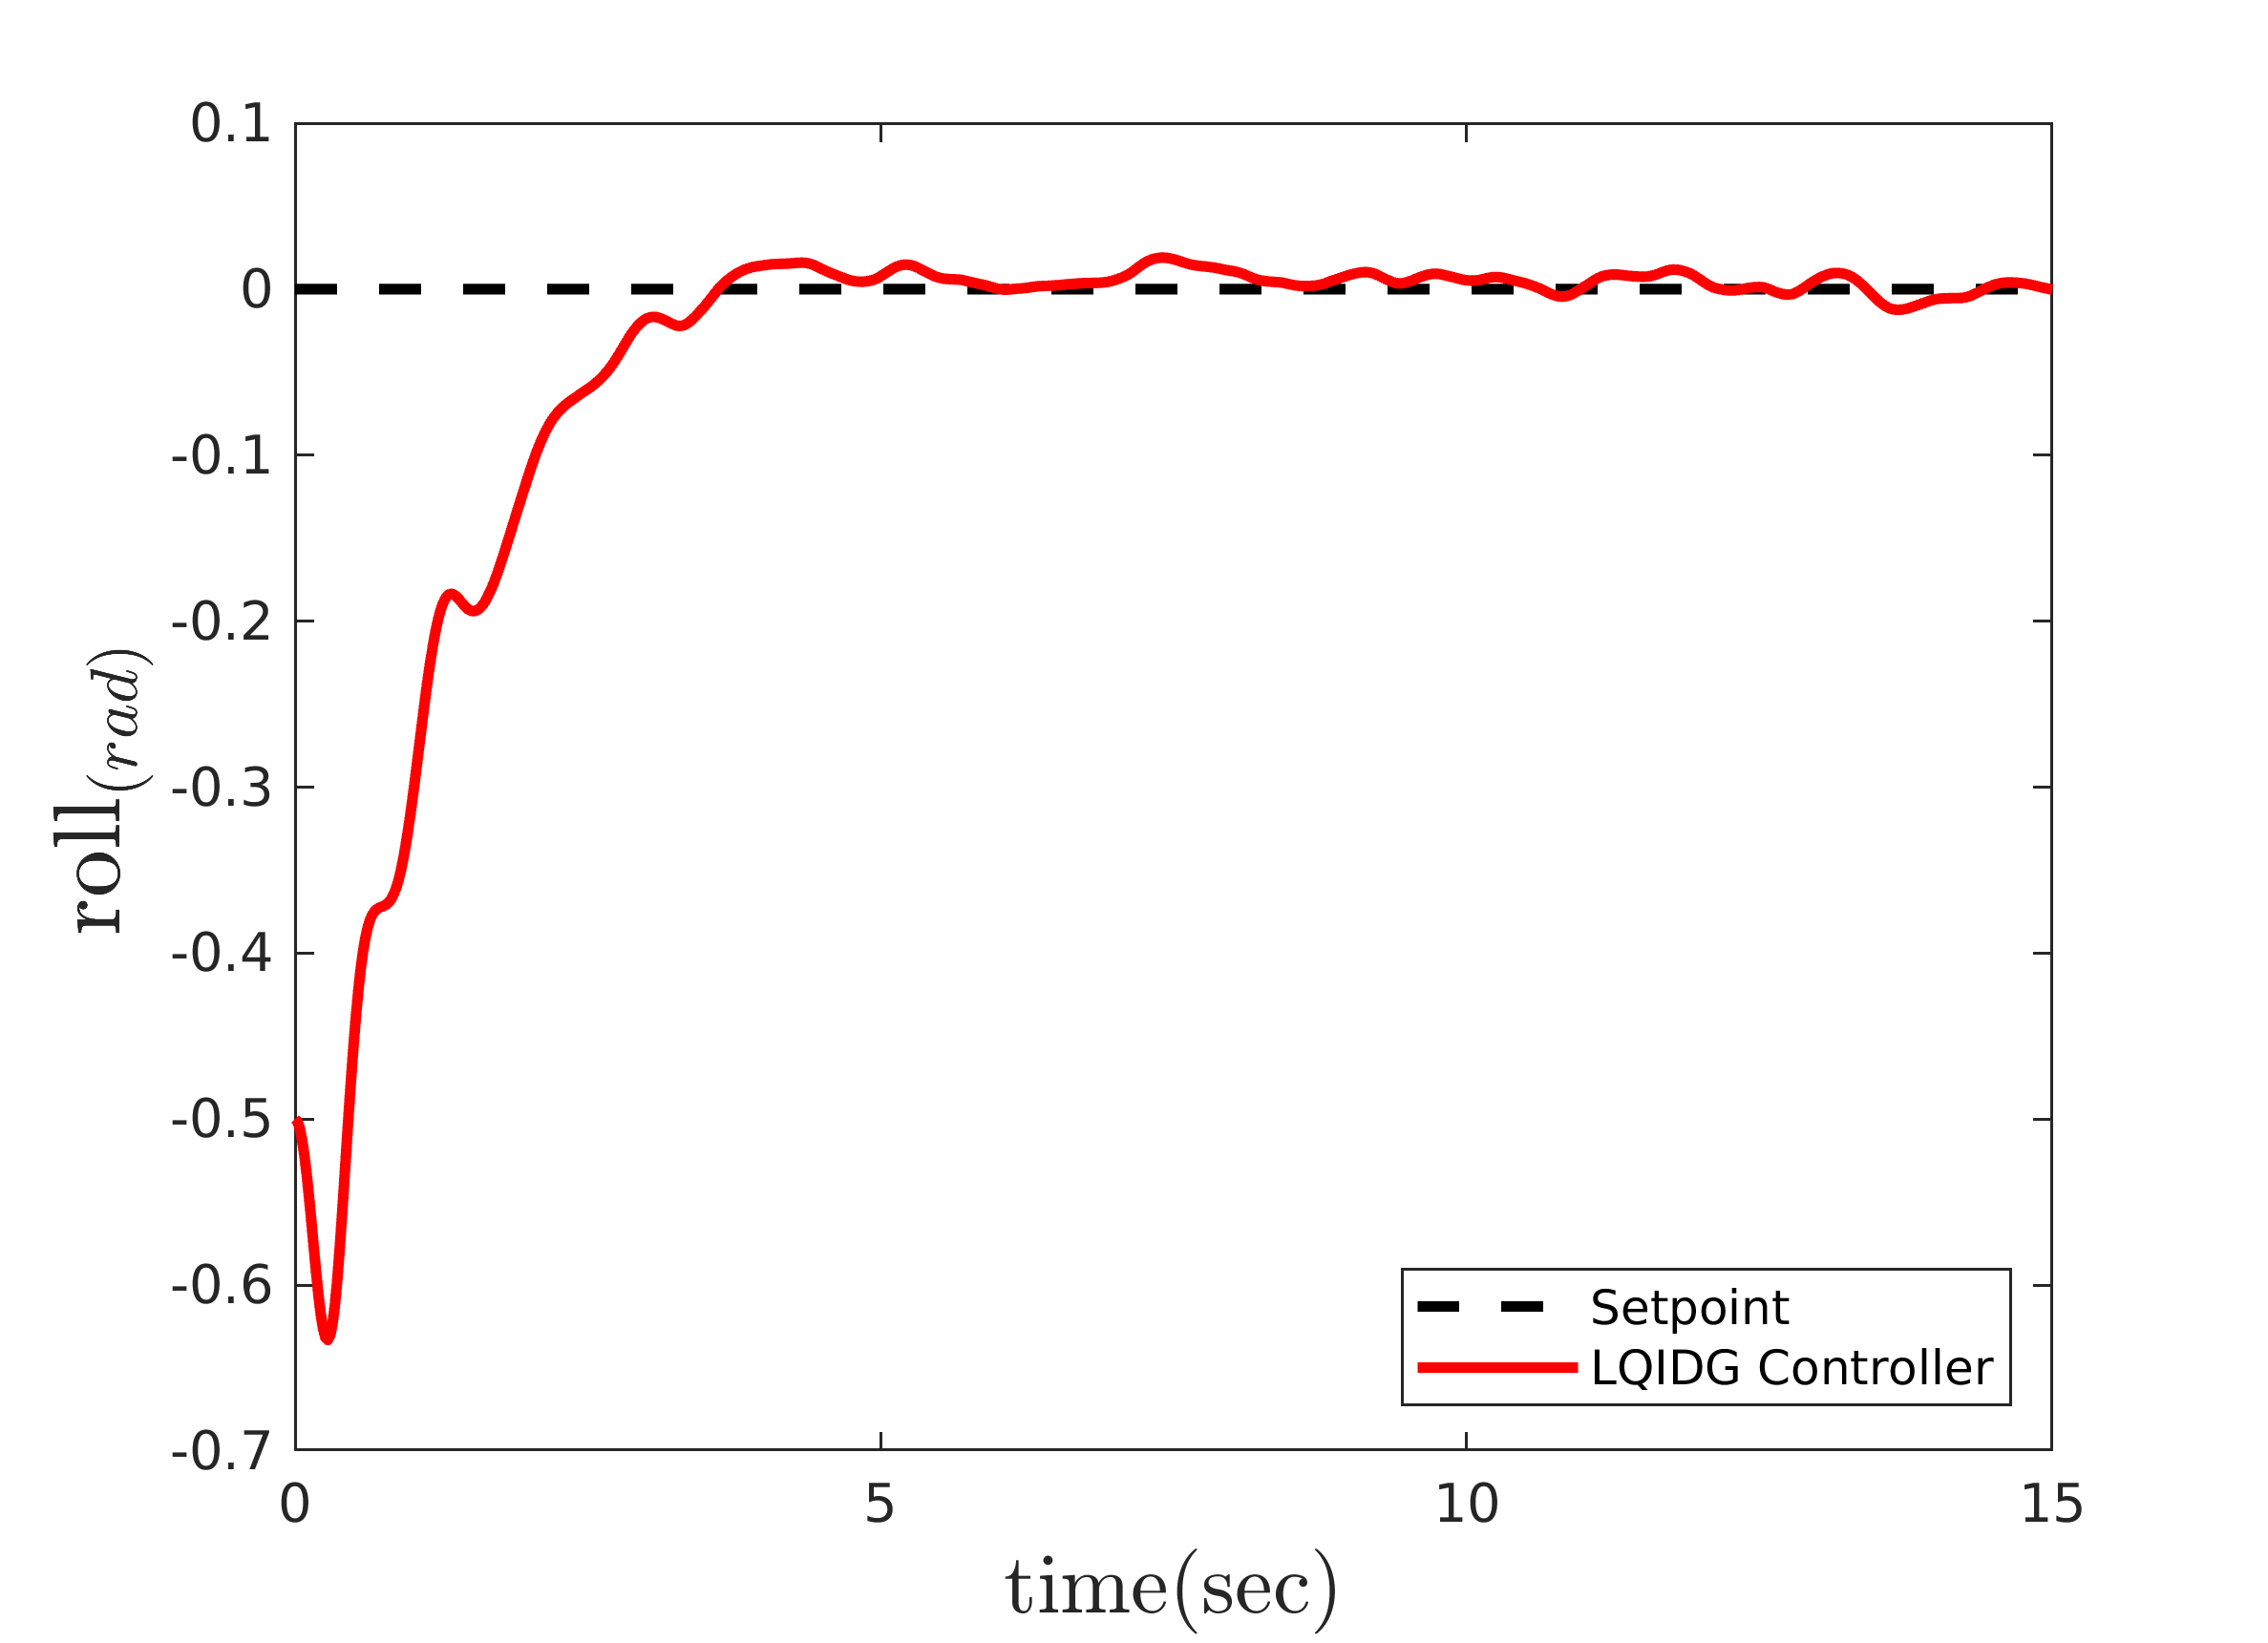
\includegraphics[width=12cm]{../Figures/MIL/LQIDG/3DOF/lqidg_roll.png}
%		\caption{تغییرات زاویه رول}
%	\end{subfigure}%
%	\begin{subfigure}
%		\centering
%		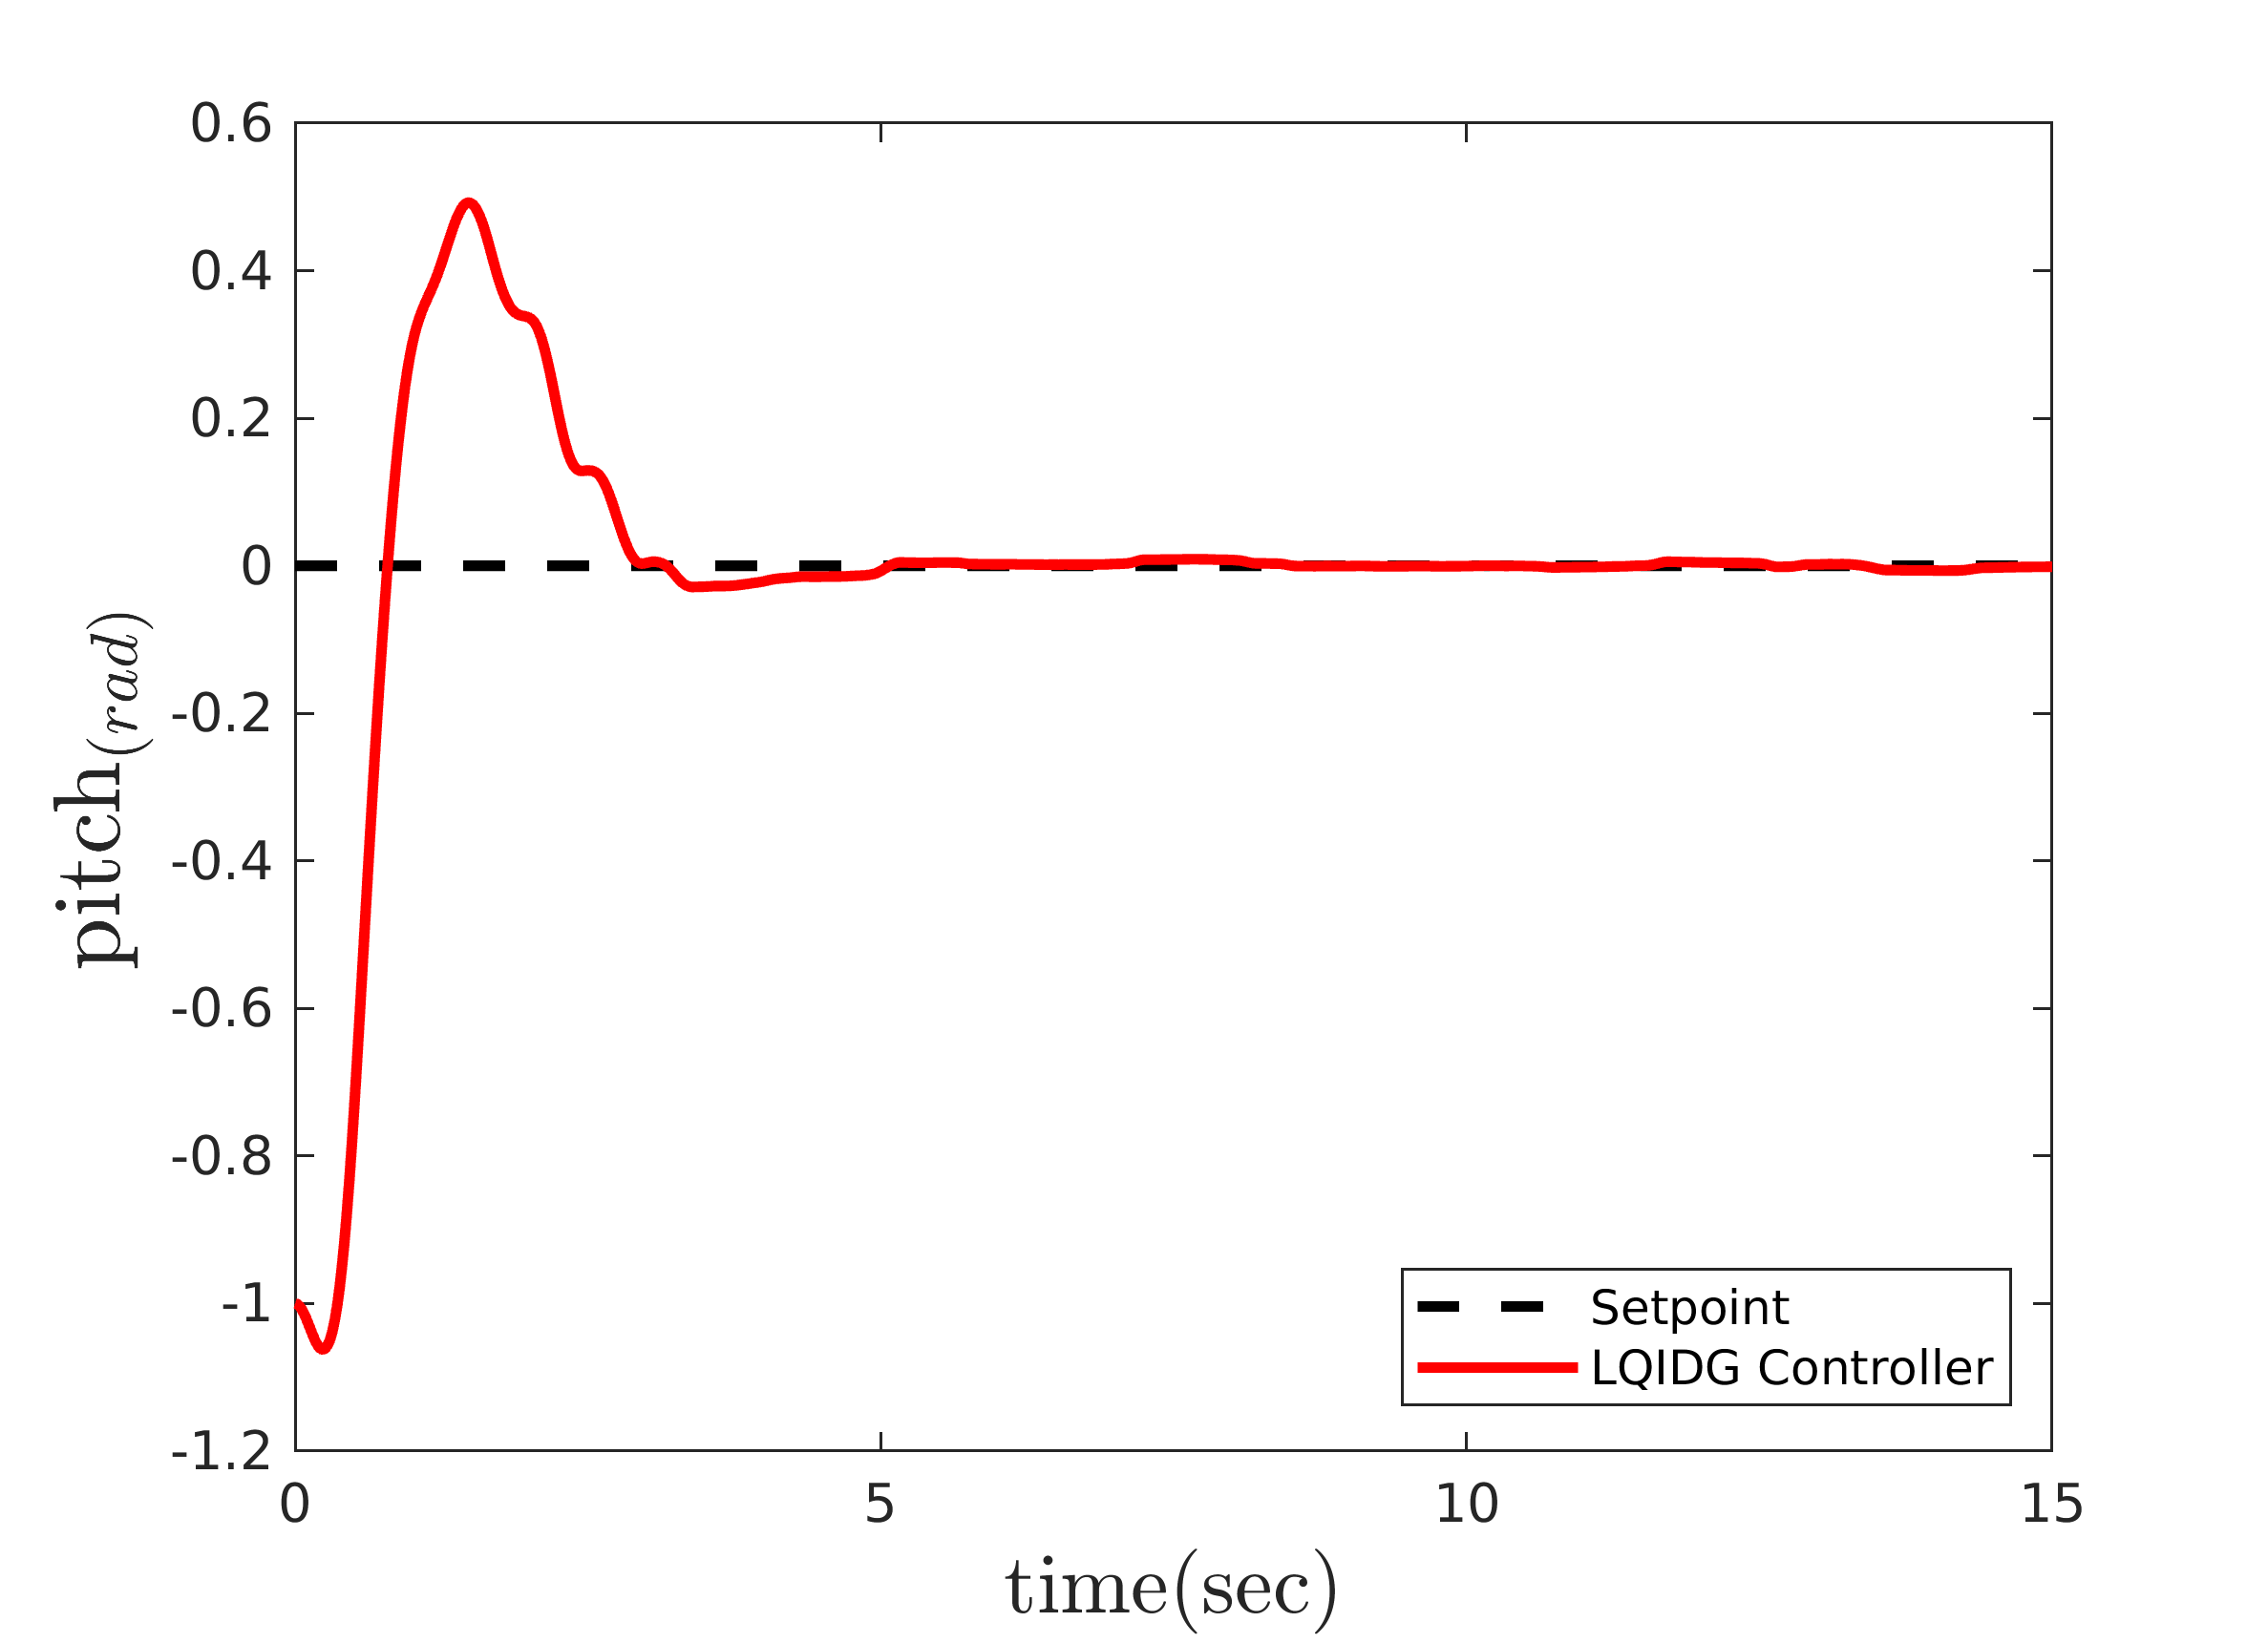
\includegraphics[width=12cm]{../Figures/MIL/LQIDG/3DOF/lqidg_pitch.png}
%		\caption{تغییرات زاویه پیچ}
%	\end{subfigure}
%	\caption{‫‪عملکرد کنترل‌کننده LQIDG در کنترل زاویه رول، پیچ و یاد (تعقیب ورودی صفر)}
%\end{figure}
%
%\begin{figure}[H]
%	\centering
%	\begin{subfigure}[H]
%		\centering
%		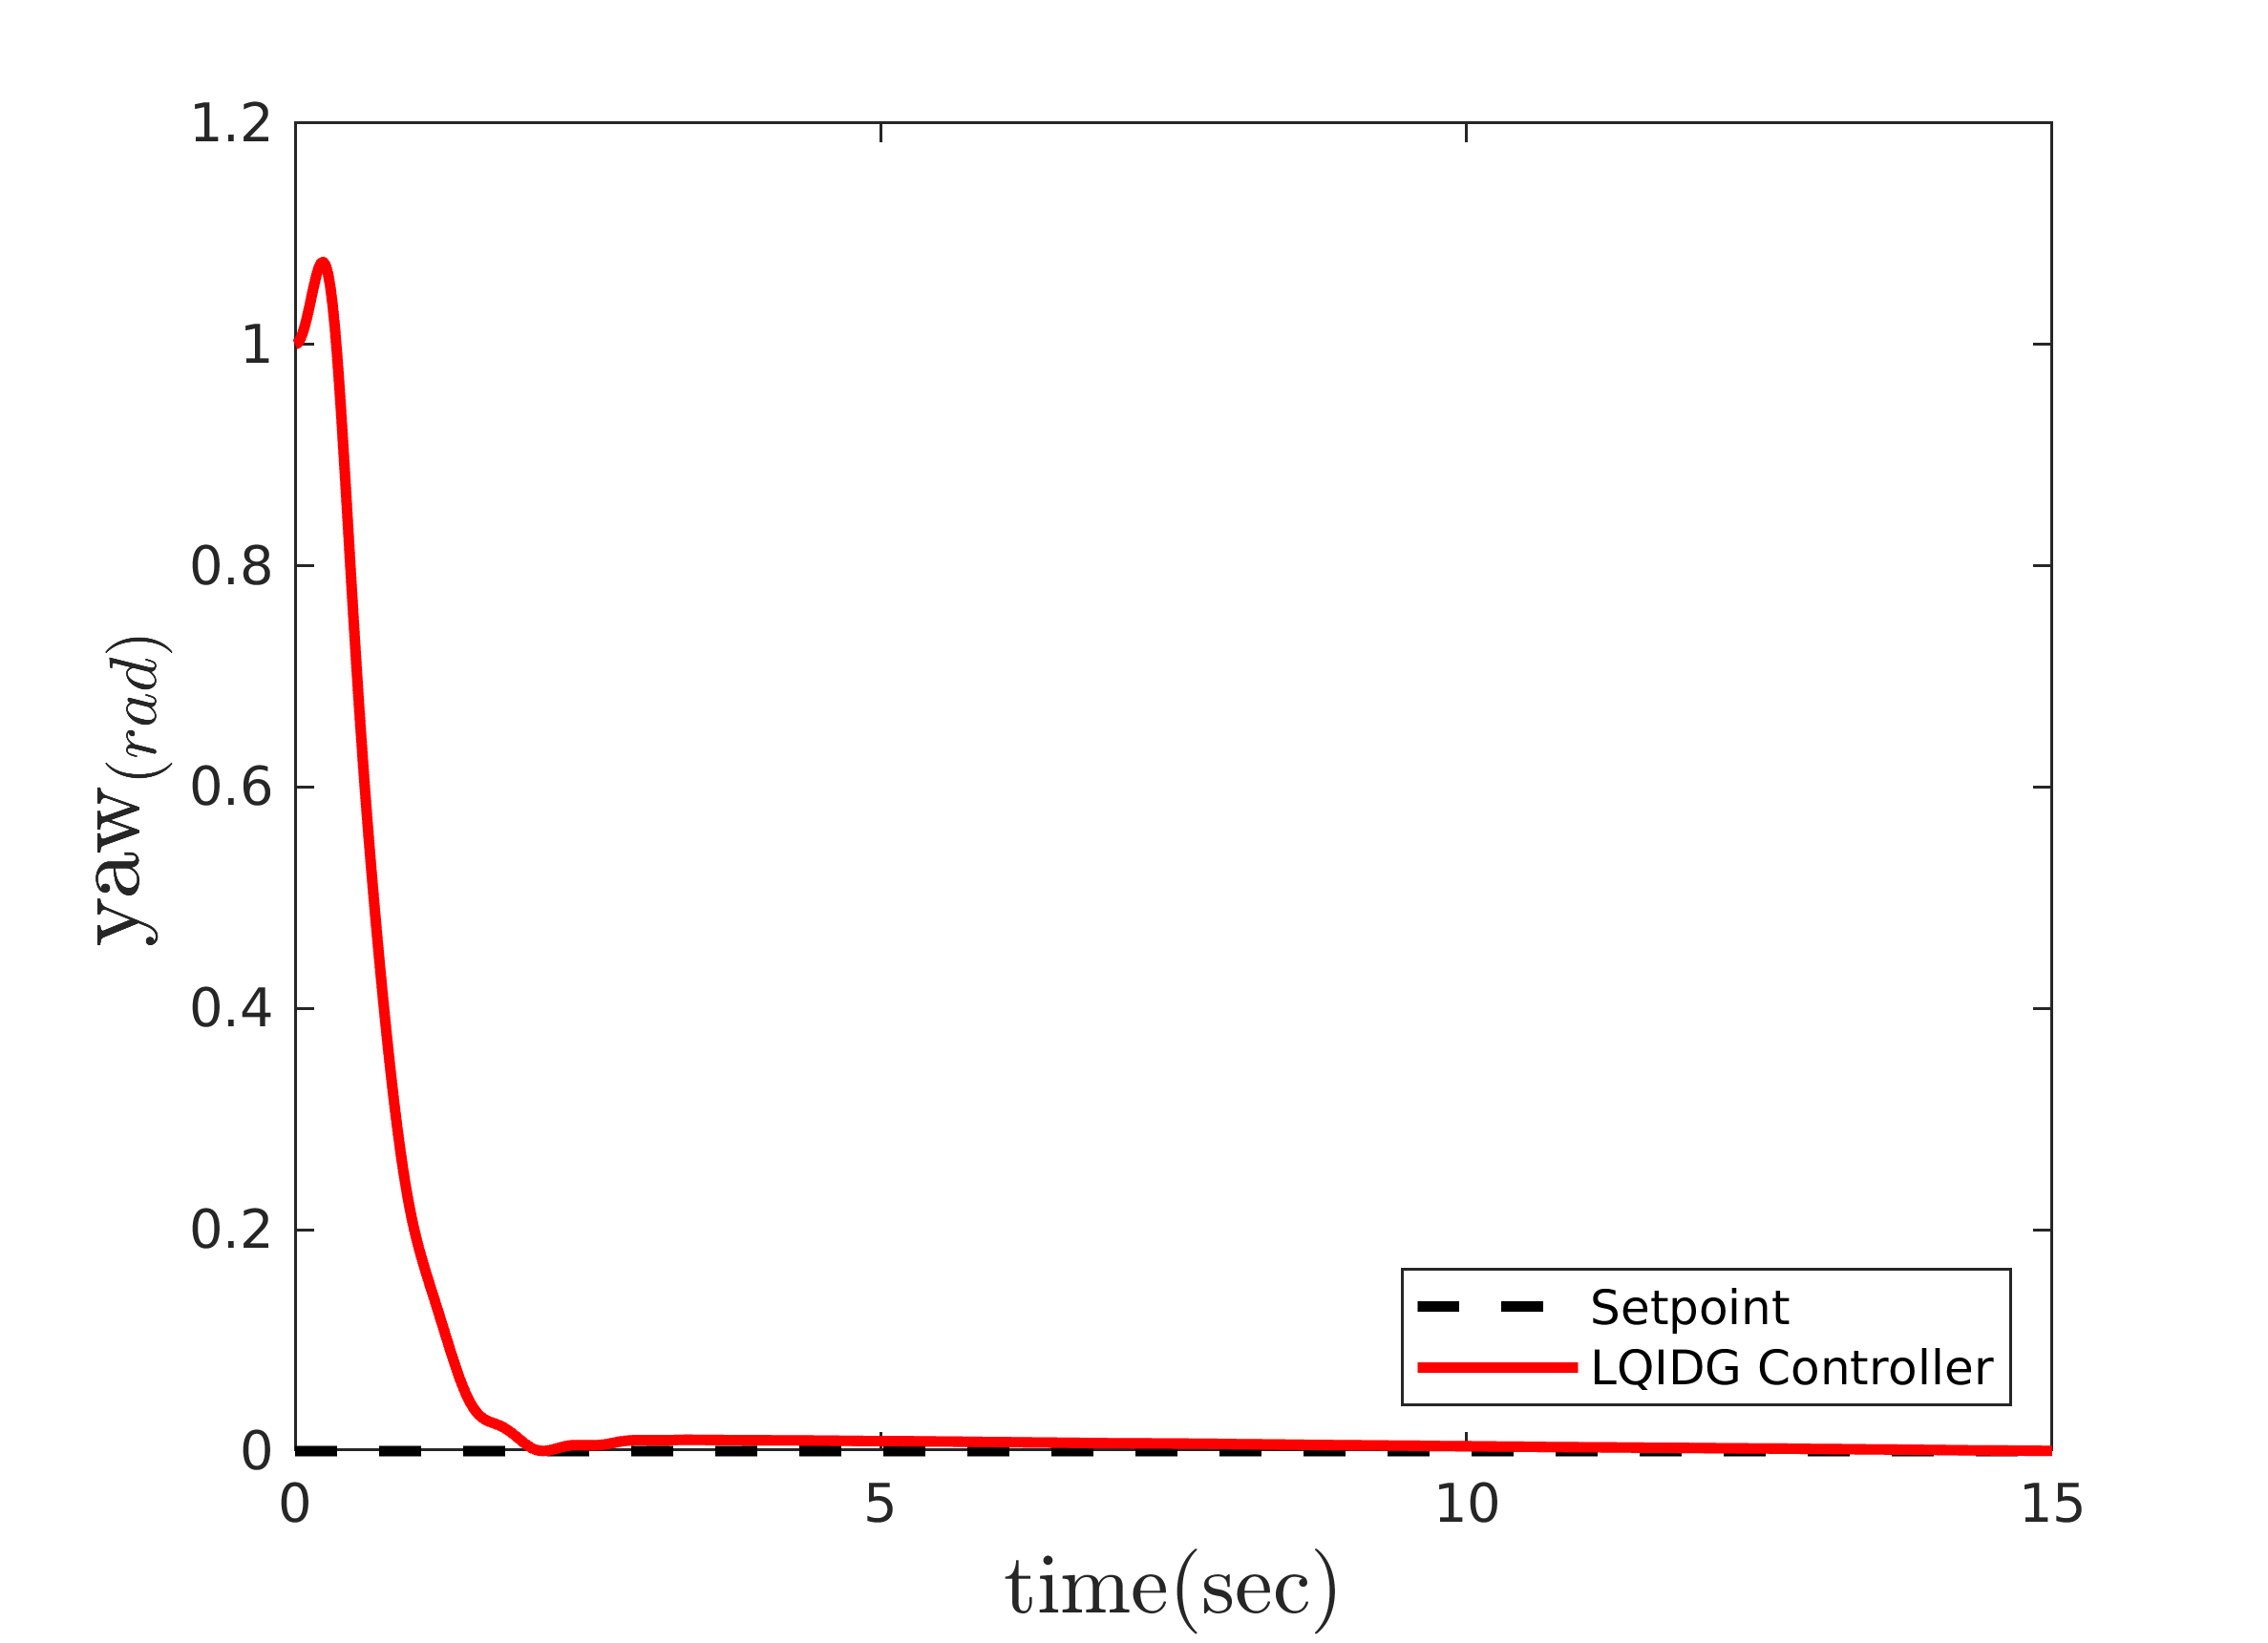
\includegraphics[width=12cm]{../Figures/MIL/LQIDG/3DOF/lqidg_yaw.png}
%		\caption{تغییرات زاویه یاو}
%	\end{subfigure}
%	\caption{‫‪عملکرد کنترل‌کننده LQIDG در کنترل زاویه رول، پیچ و یاد (تعقیب ورودی صفر)}
%\end{figure}
\begin{figure}[H]
	\centering
\subfigure[تغییرات زاویه رول]{
	\centering
	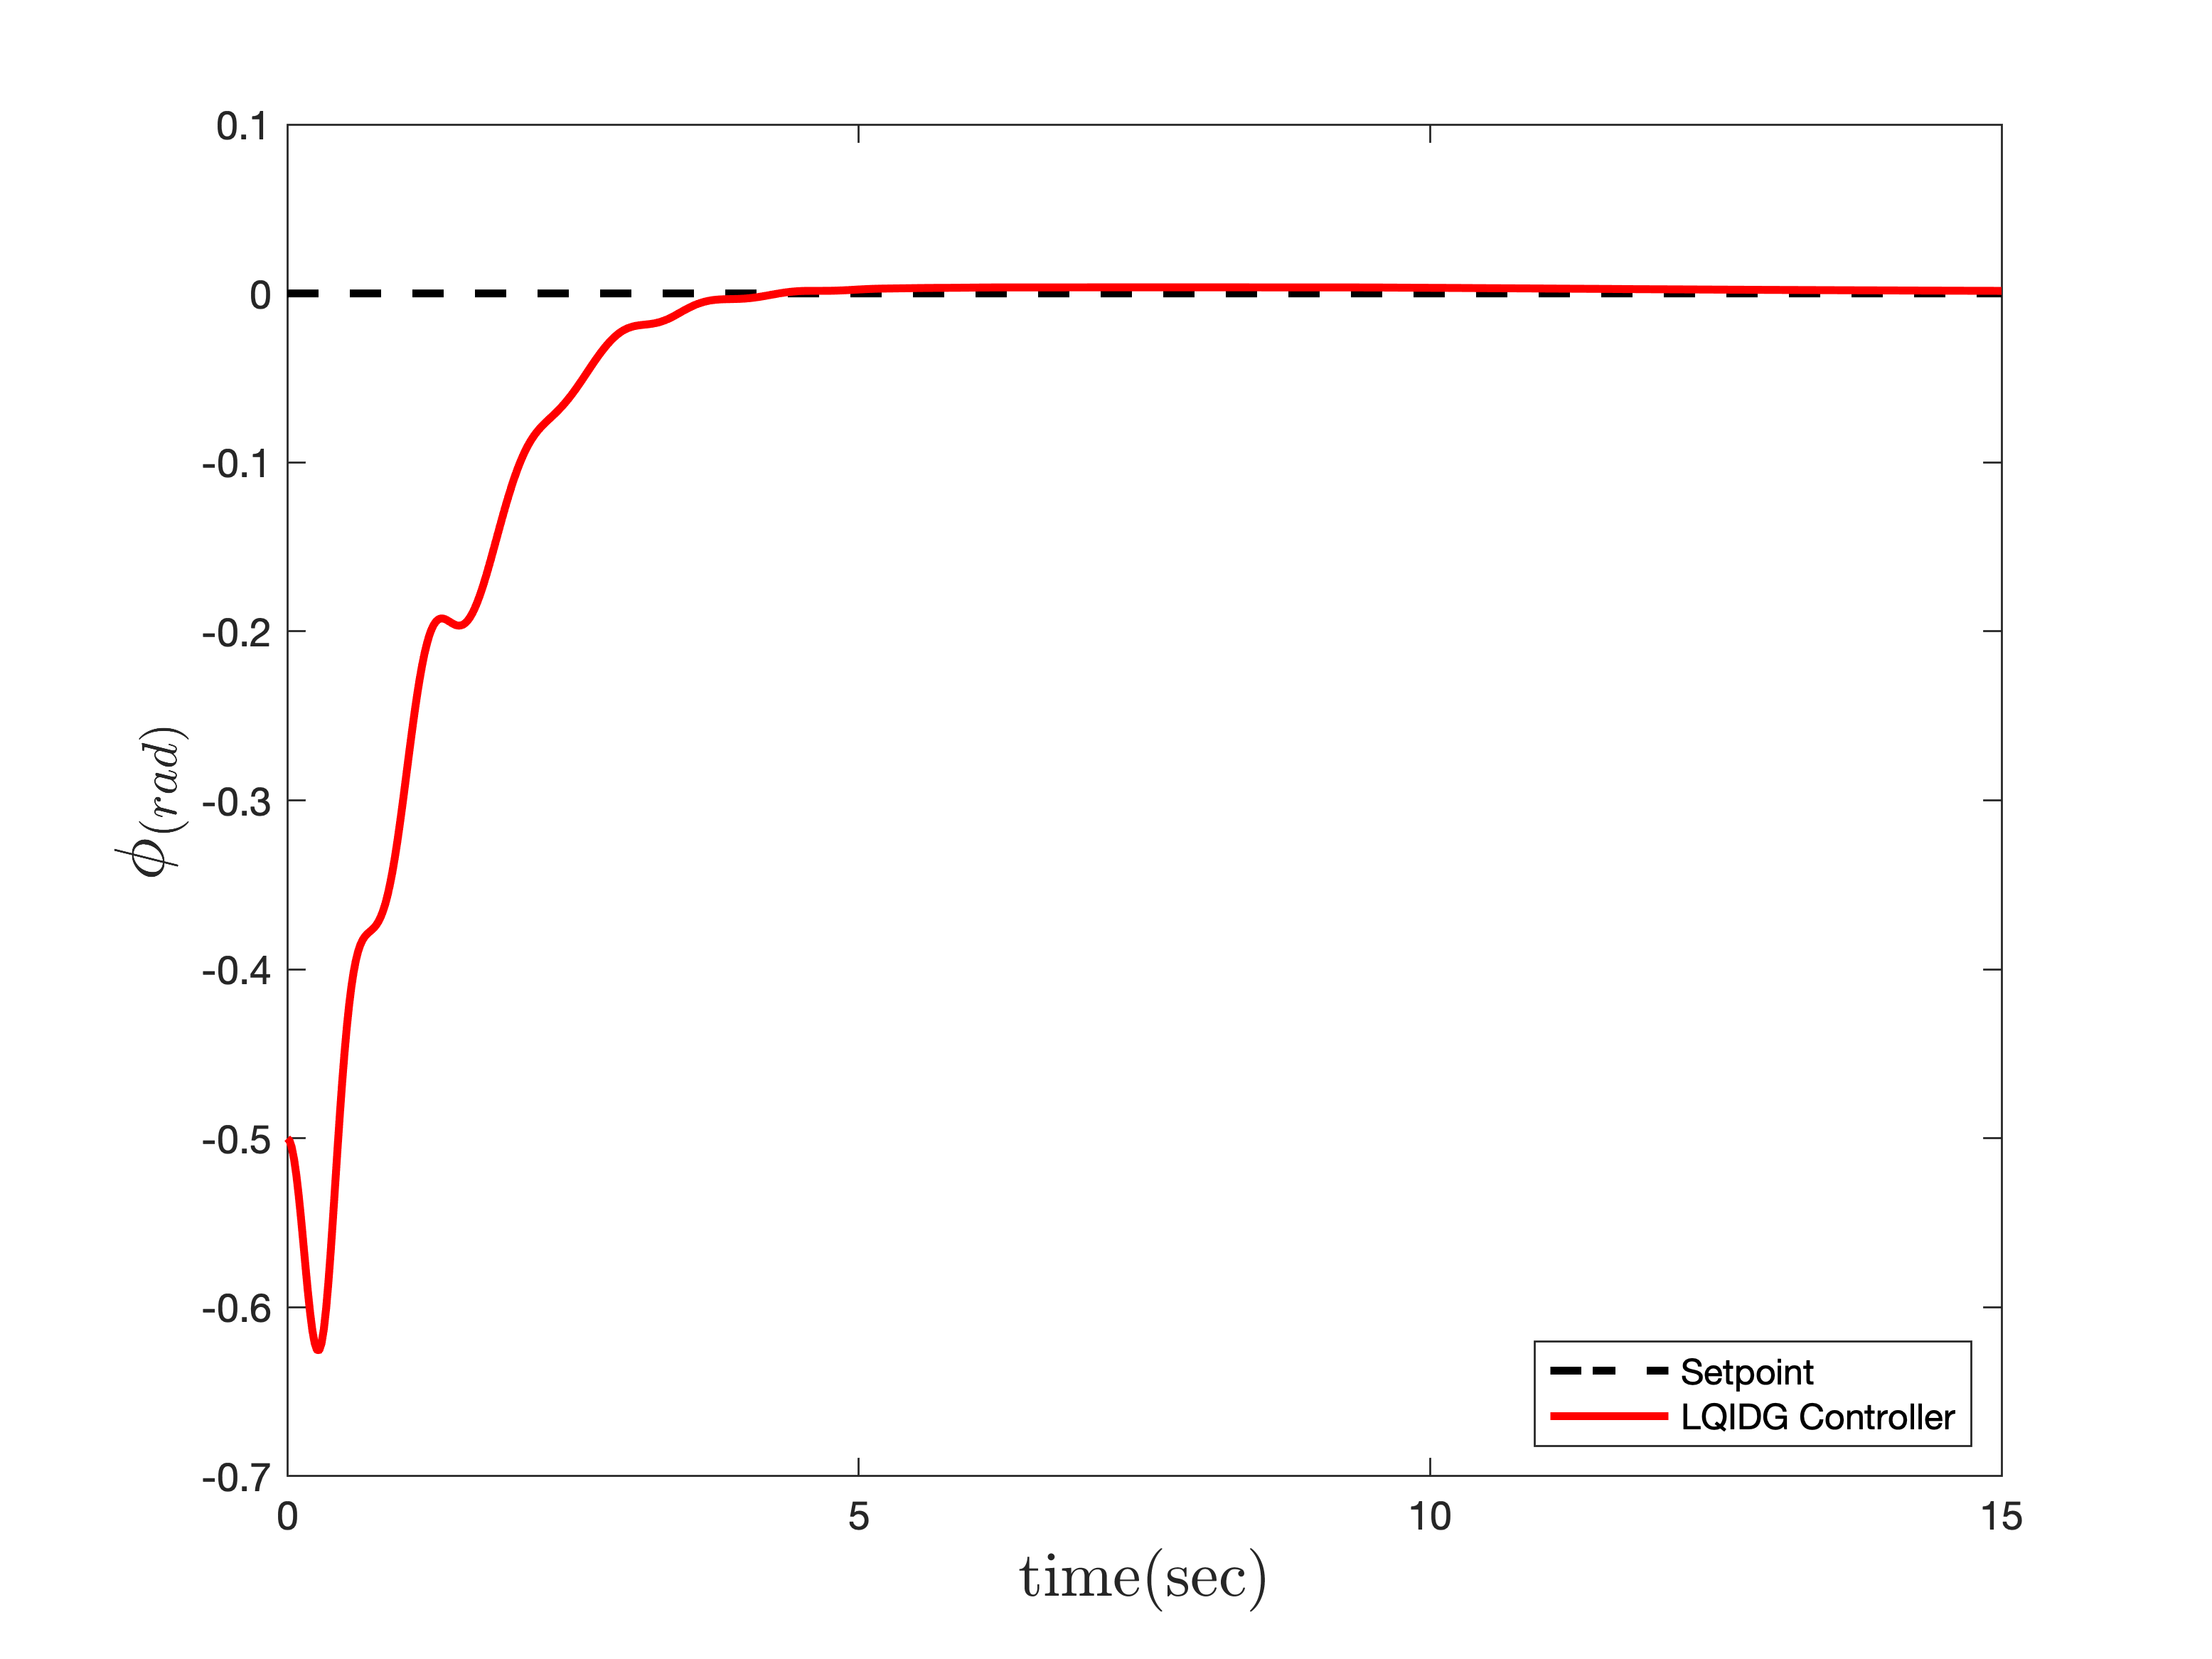
\includegraphics[width=.48\linewidth]{../Figures/MIL/LQIDG/3DOF/lqidg_roll_nn.png}
}
\subfigure[تغییرات زاویه پیچ]{
	\centering
	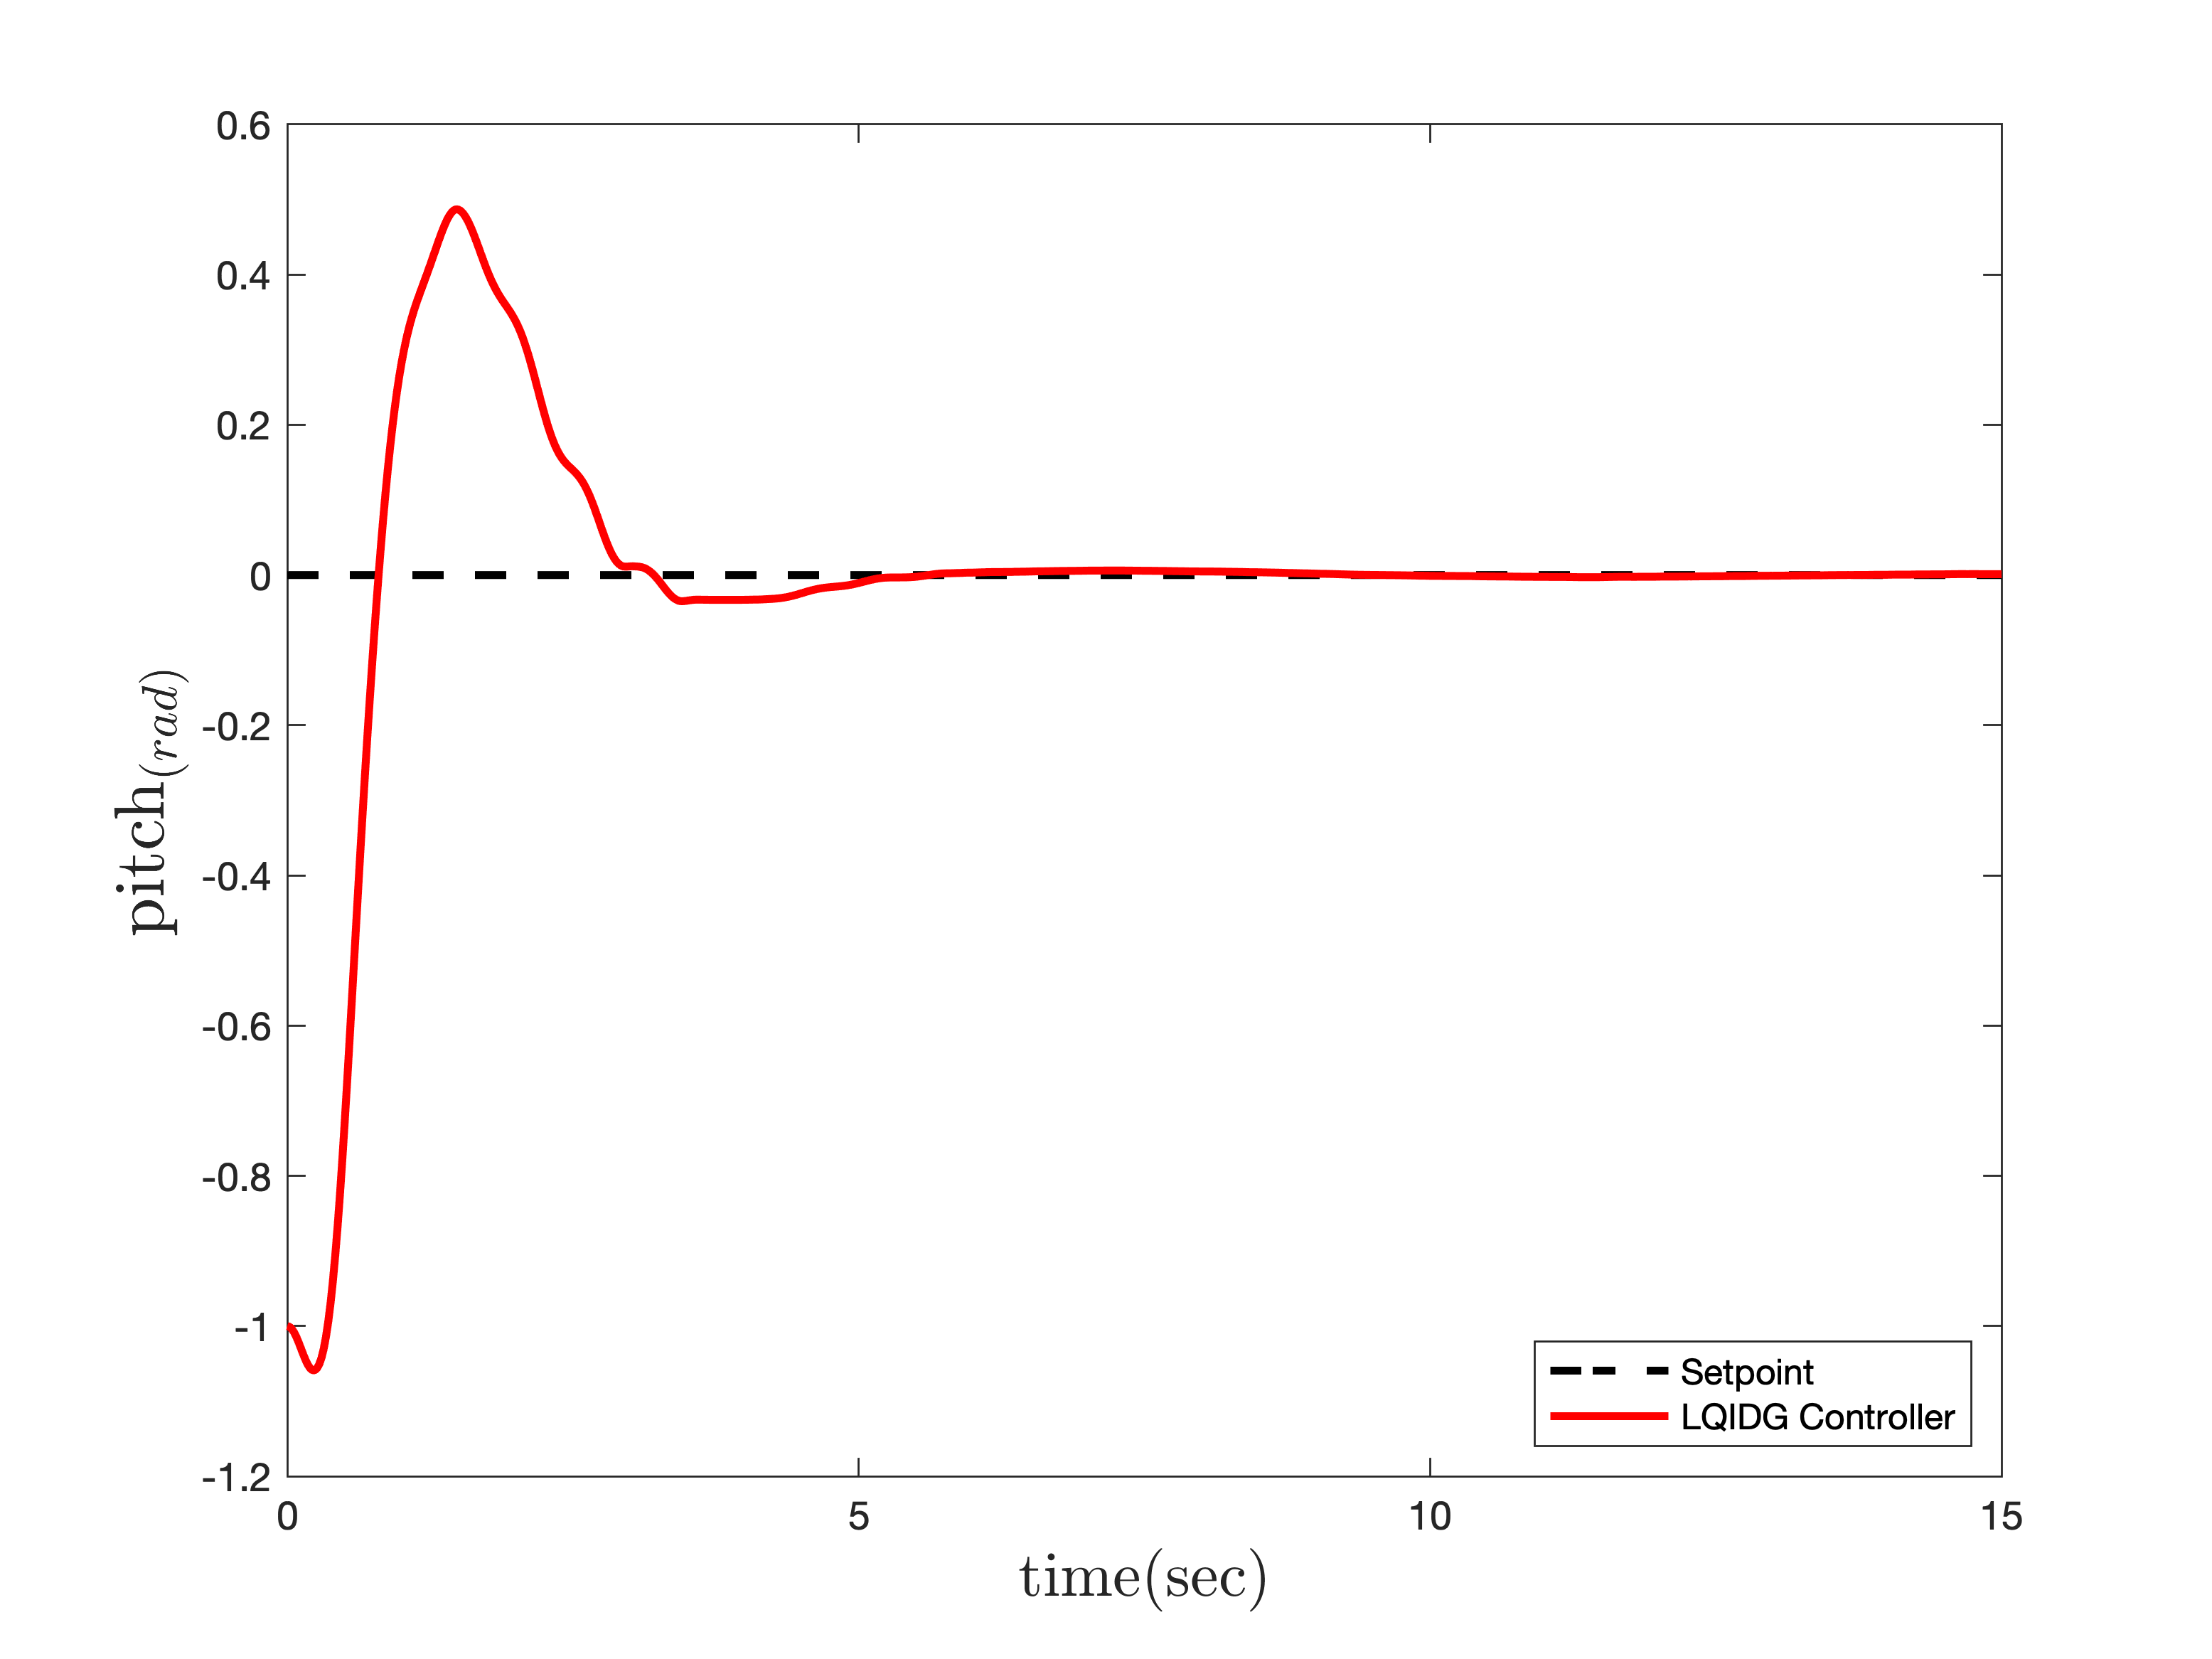
\includegraphics[width=.48\linewidth]{../Figures/MIL/LQIDG/3DOF/lqidg_pitch_nn.png}
}
\subfigure[تغییرات زاویه یاو]{
	\centering
	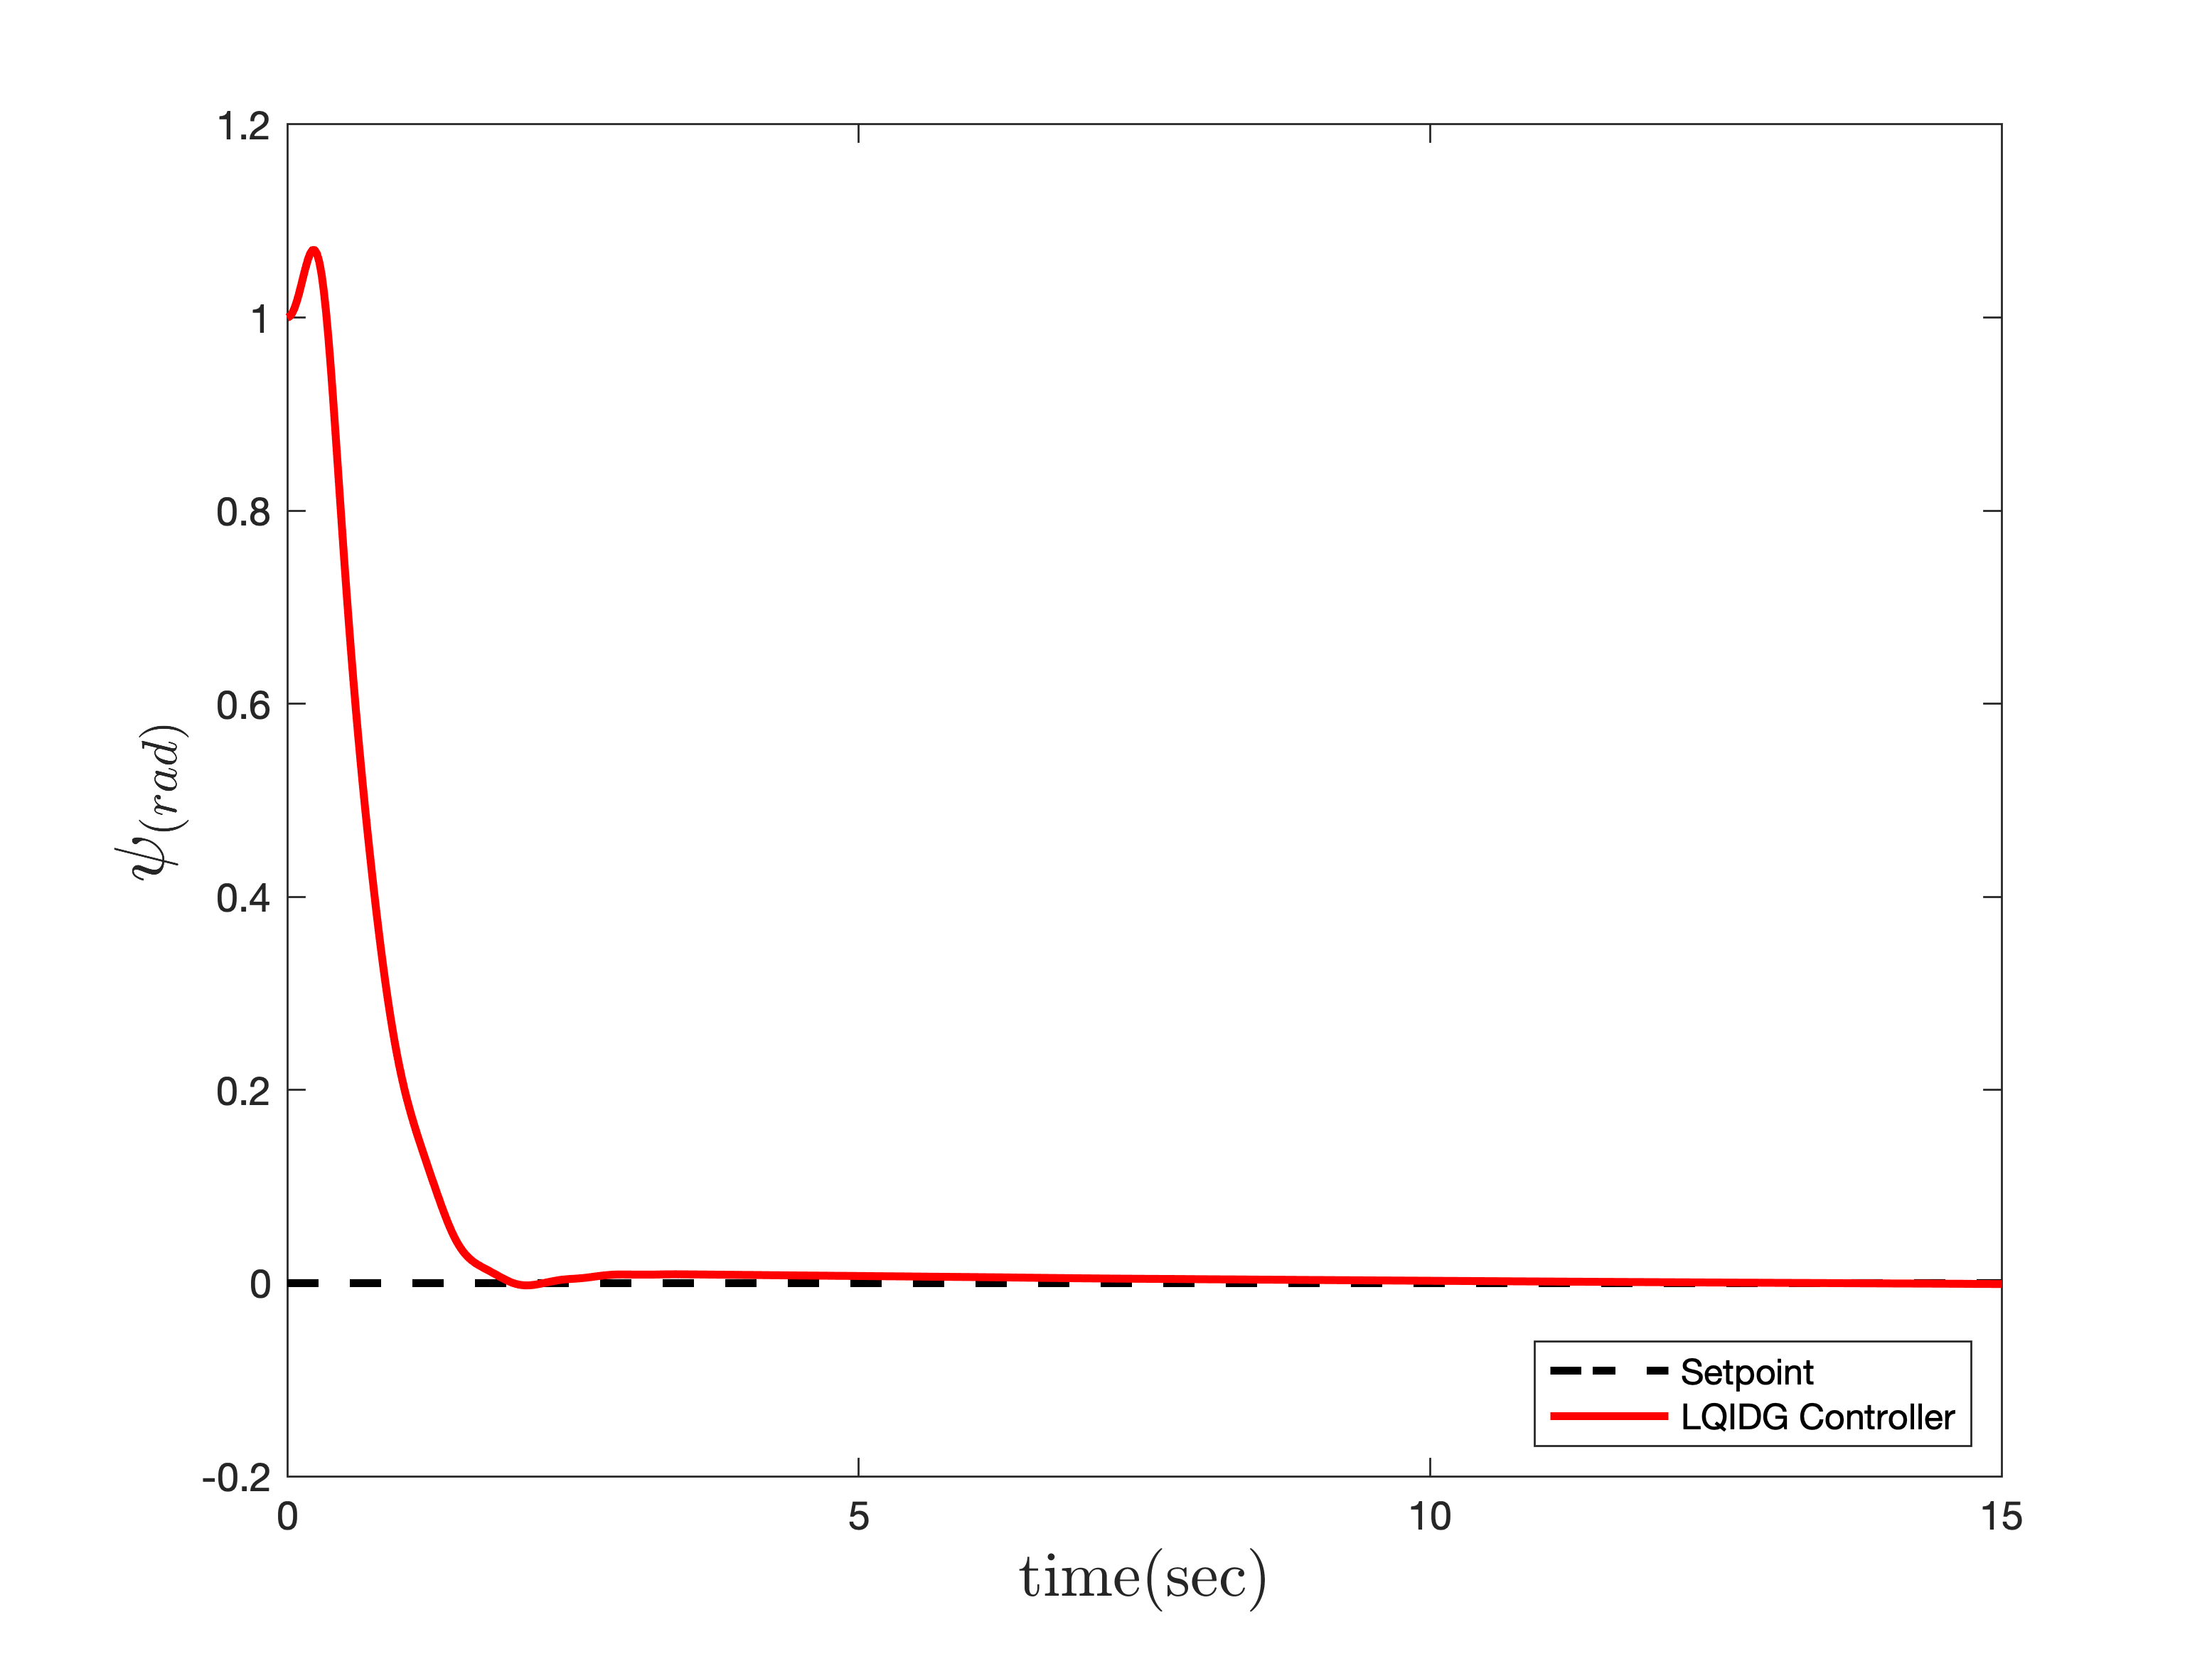
\includegraphics[width=.48\linewidth]{../Figures/MIL/LQIDG/3DOF/lqidg_yaw_nn.png}
}
	\caption{‫‪عملکرد کنترل‌کننده \lr{LQIDG} در کنترل وضعیت (تعقیب ورودی صفر)}
	\label{lqidg_roll_pitch_yaw_fig_simulation_ll}
\end{figure}
همانطور که از شکل
\ref{lqidg_roll_pitch_yaw_fig_simulation_ll}
مشخص است، زمان نشست برای کانال‌های مختلف حداکثر پنج ثانیه است. خطای مانگار ندارد. در ادامه فرمان کنترلی موتورها آورده شده‌است.

\begin{figure}[H]
	\centering
	\subfigure[موتور شماره یک]{
		\centering
		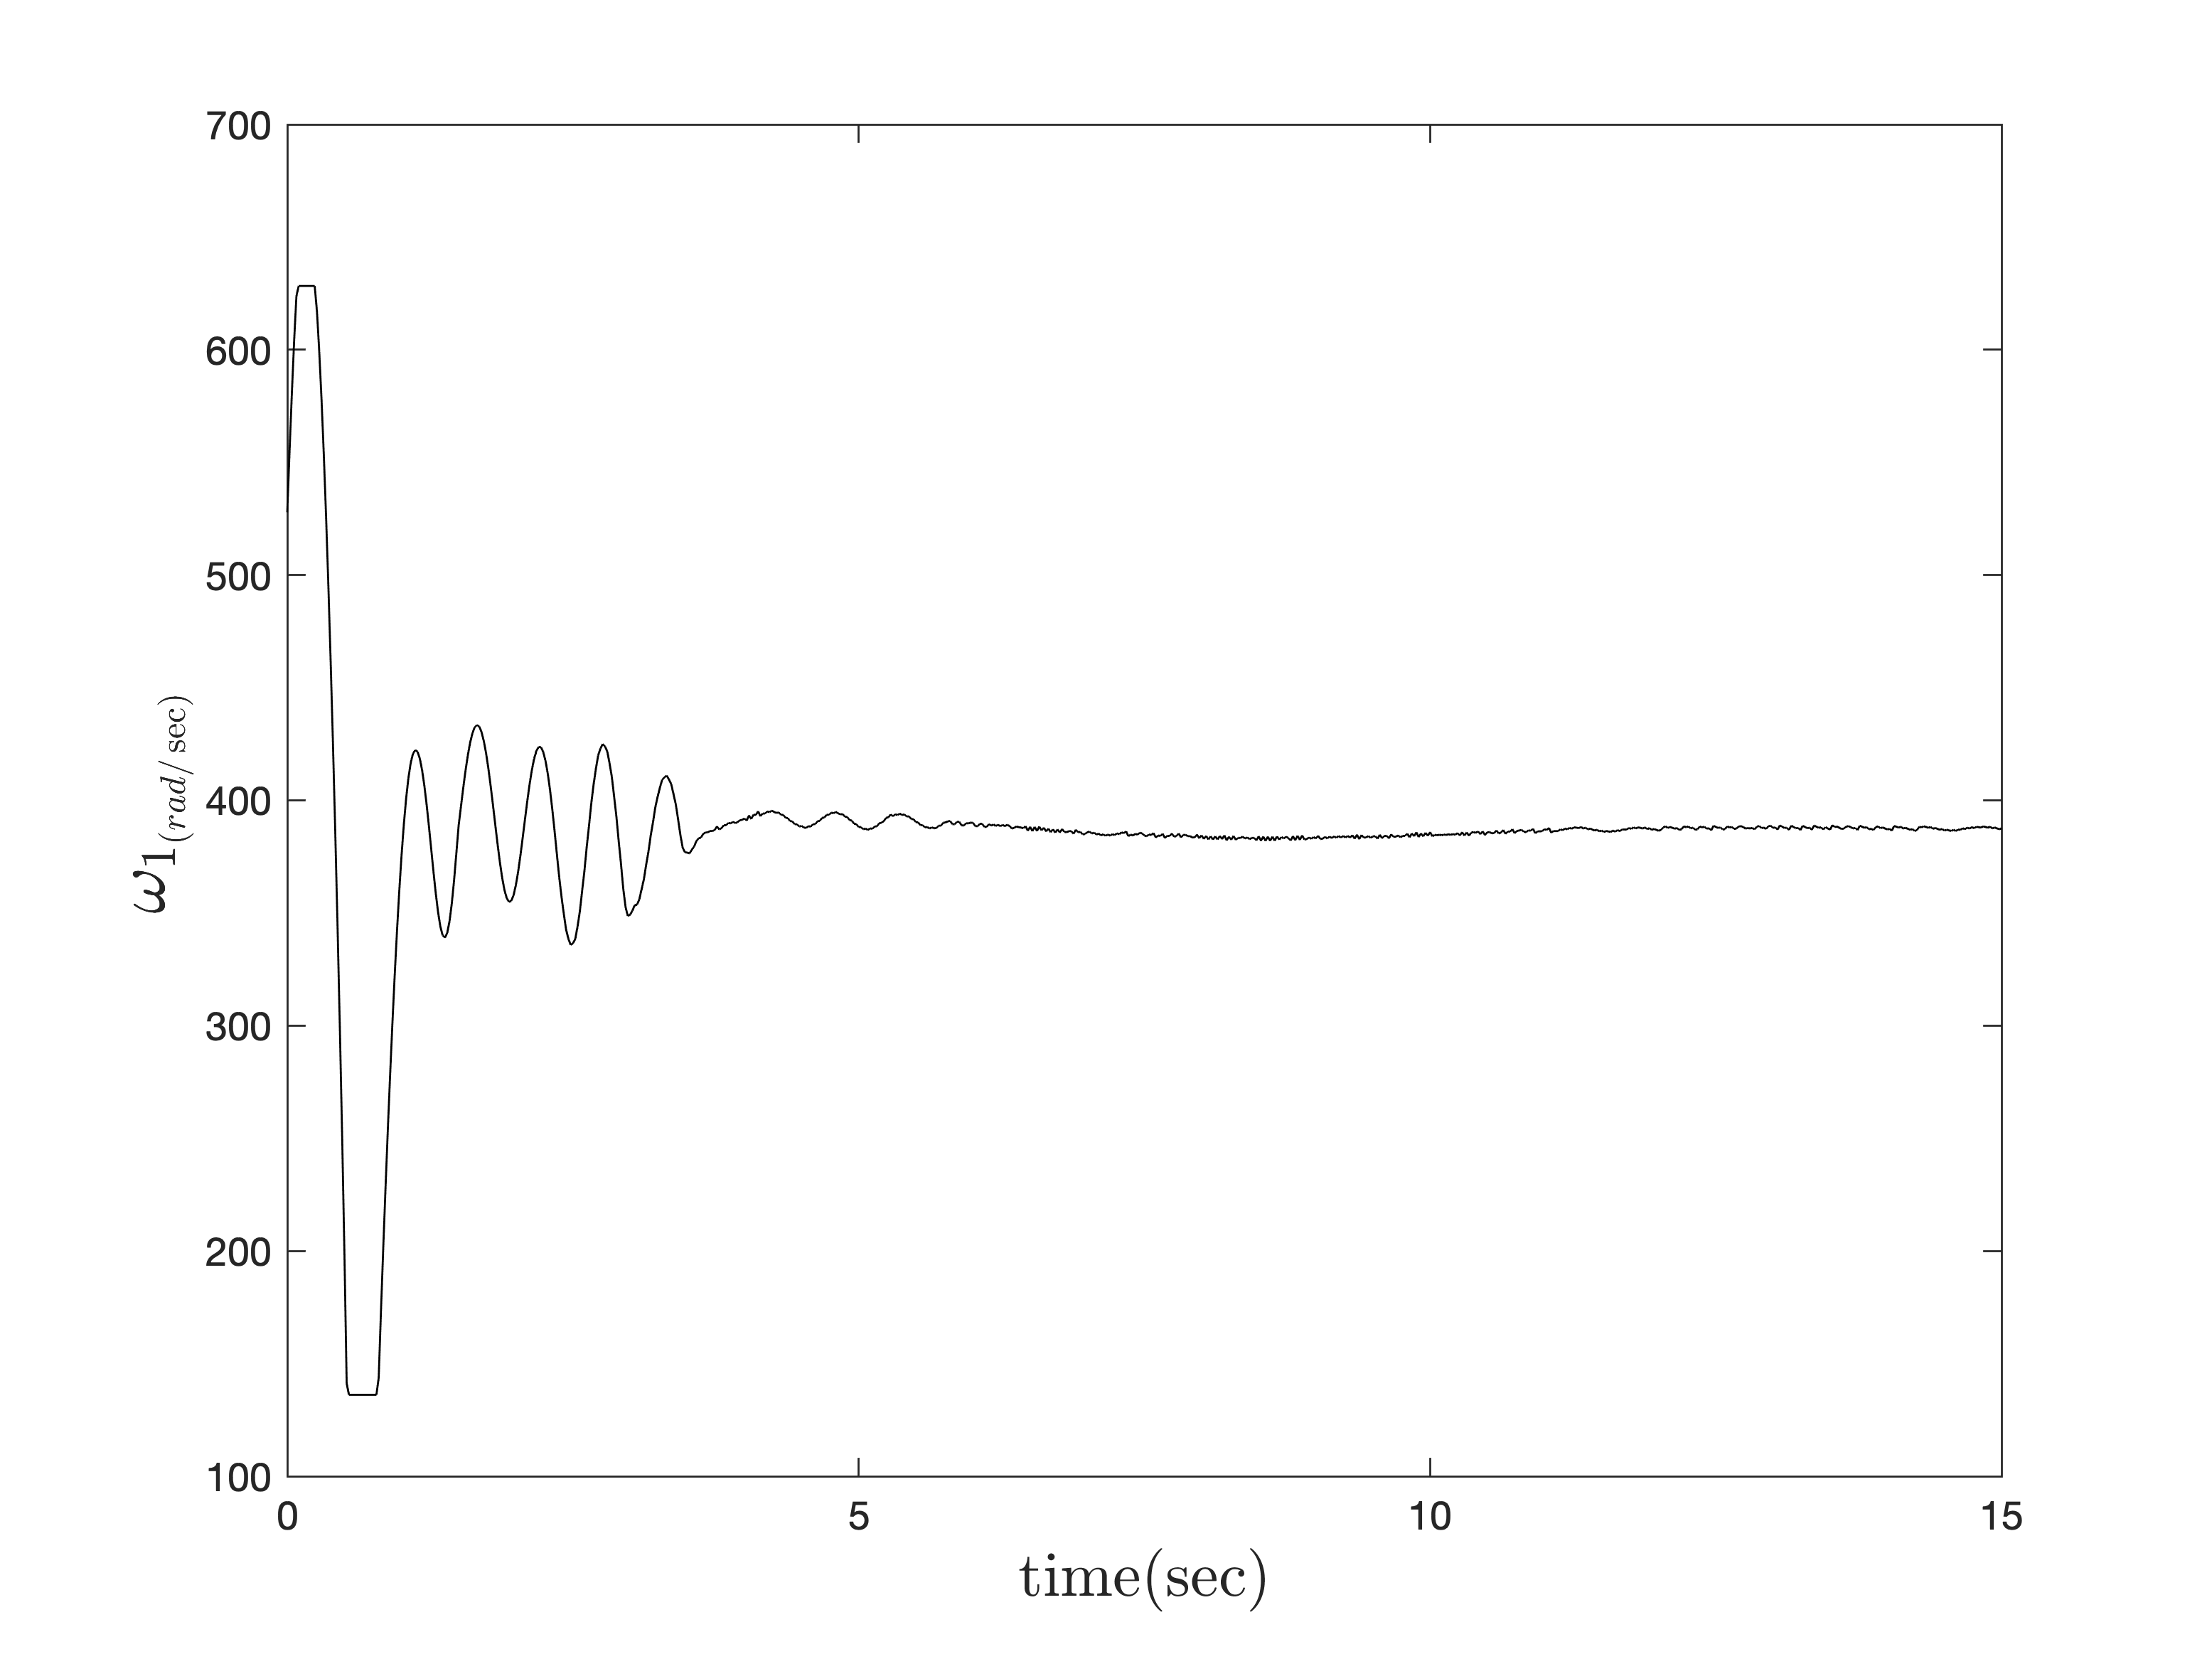
\includegraphics[width=.45\linewidth]{../Figures/MIL/LQIDG/3DOF/lqidg_roll_pitch_Omega_1_nn.png}
	}
	\subfigure[موتور شماره دو]{
		\centering
		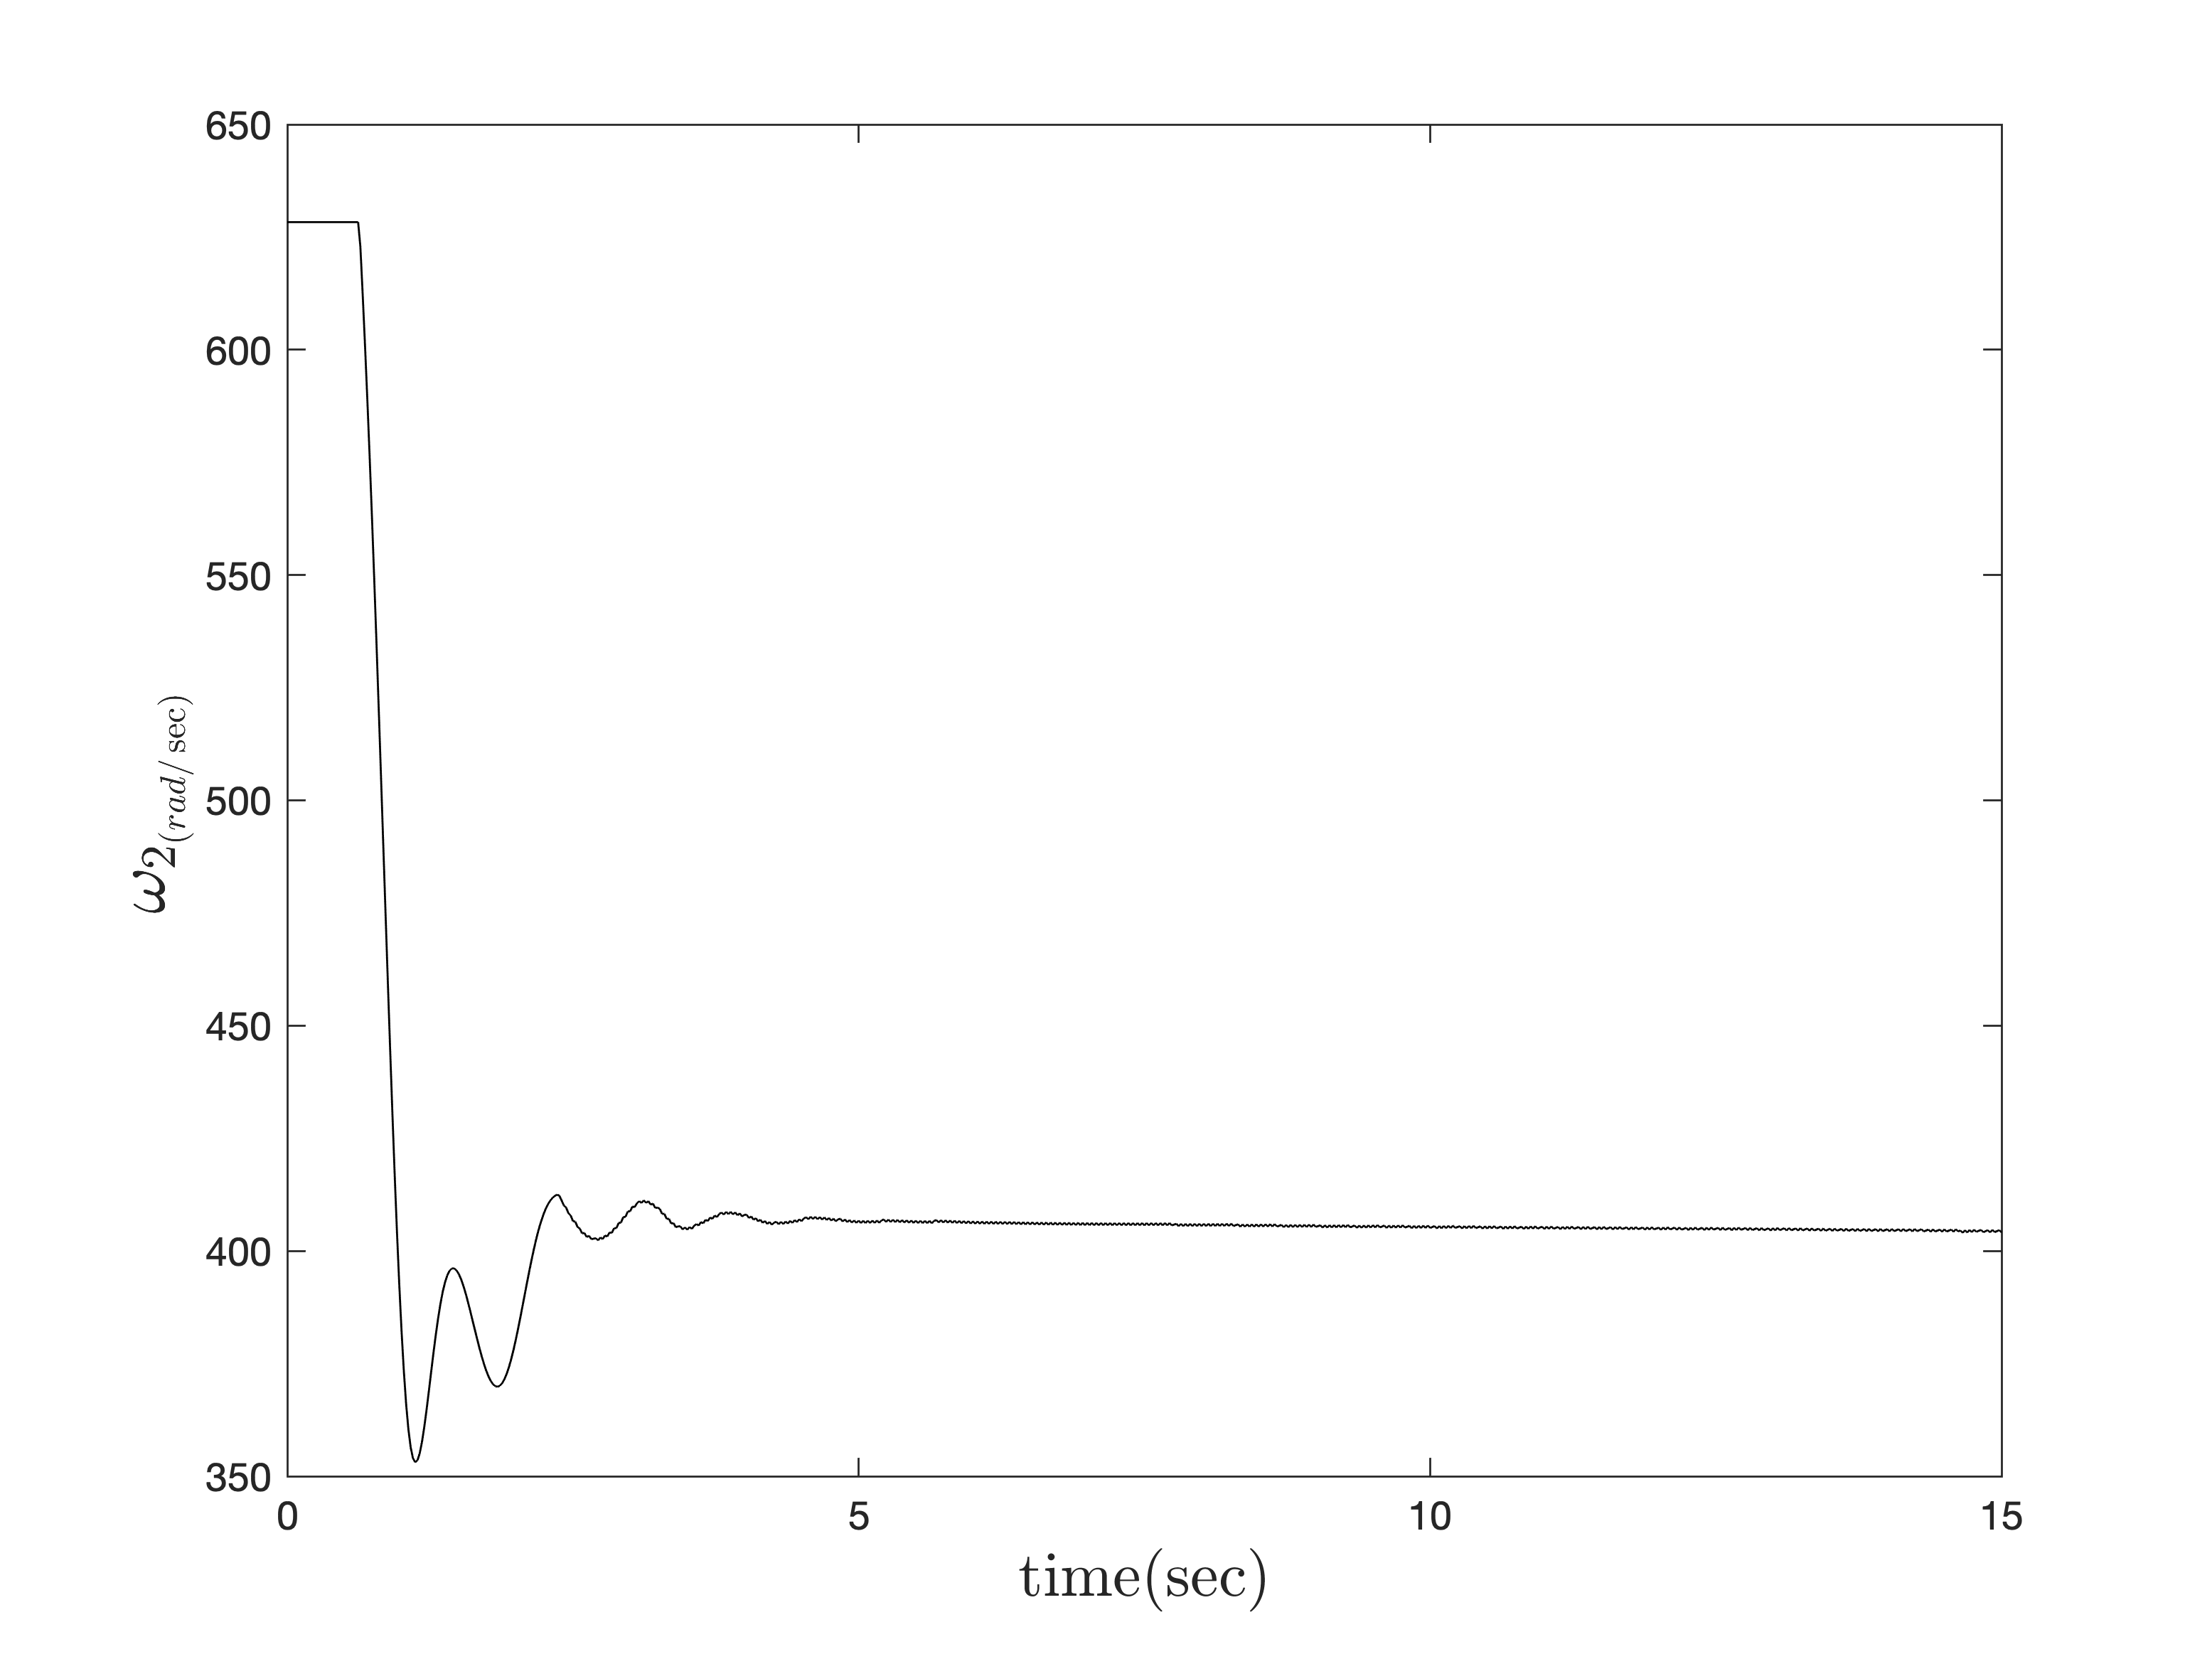
\includegraphics[width=.45\linewidth]{../Figures/MIL/LQIDG/3DOF/lqidg_roll_pitch_Omega_2_nn.png}
	}
	\subfigure[موتور شماره سه]{
		\centering
		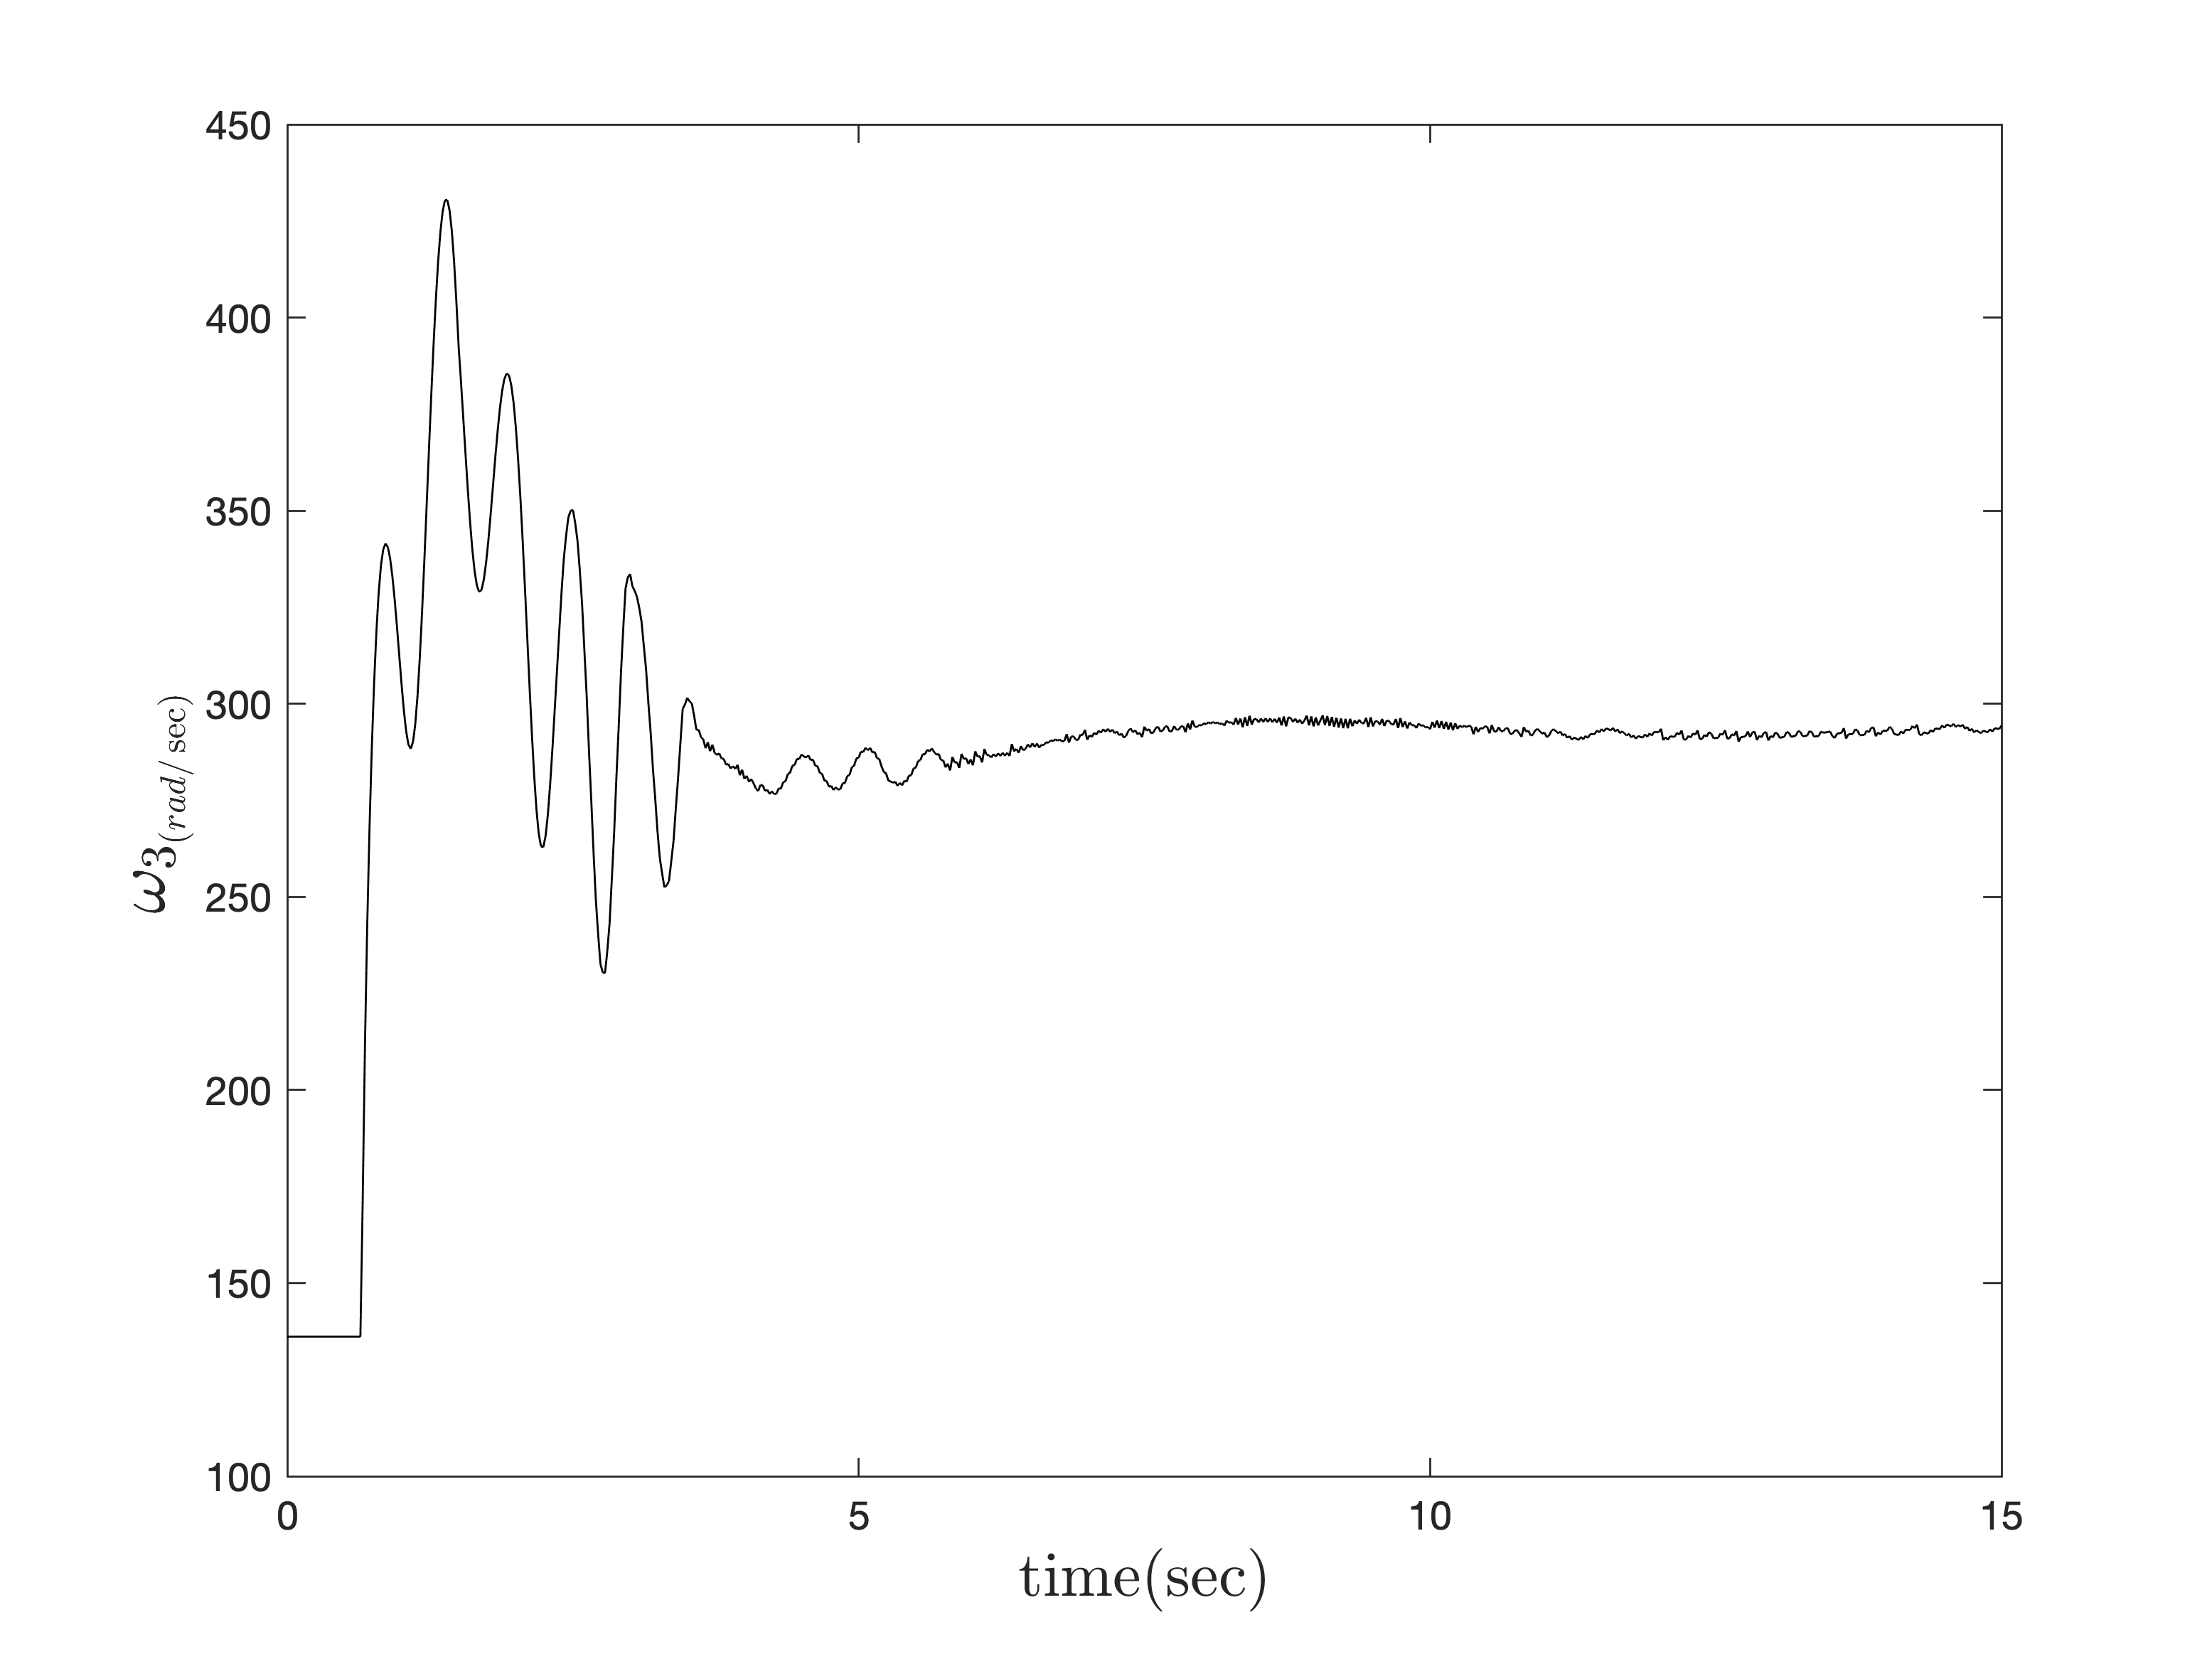
\includegraphics[width=.45\linewidth]{../Figures/MIL/LQIDG/3DOF/lqidg_roll_pitch_Omega_3_nn.png}
	}
	\subfigure[موتور شماره چهار]{
		\centering
		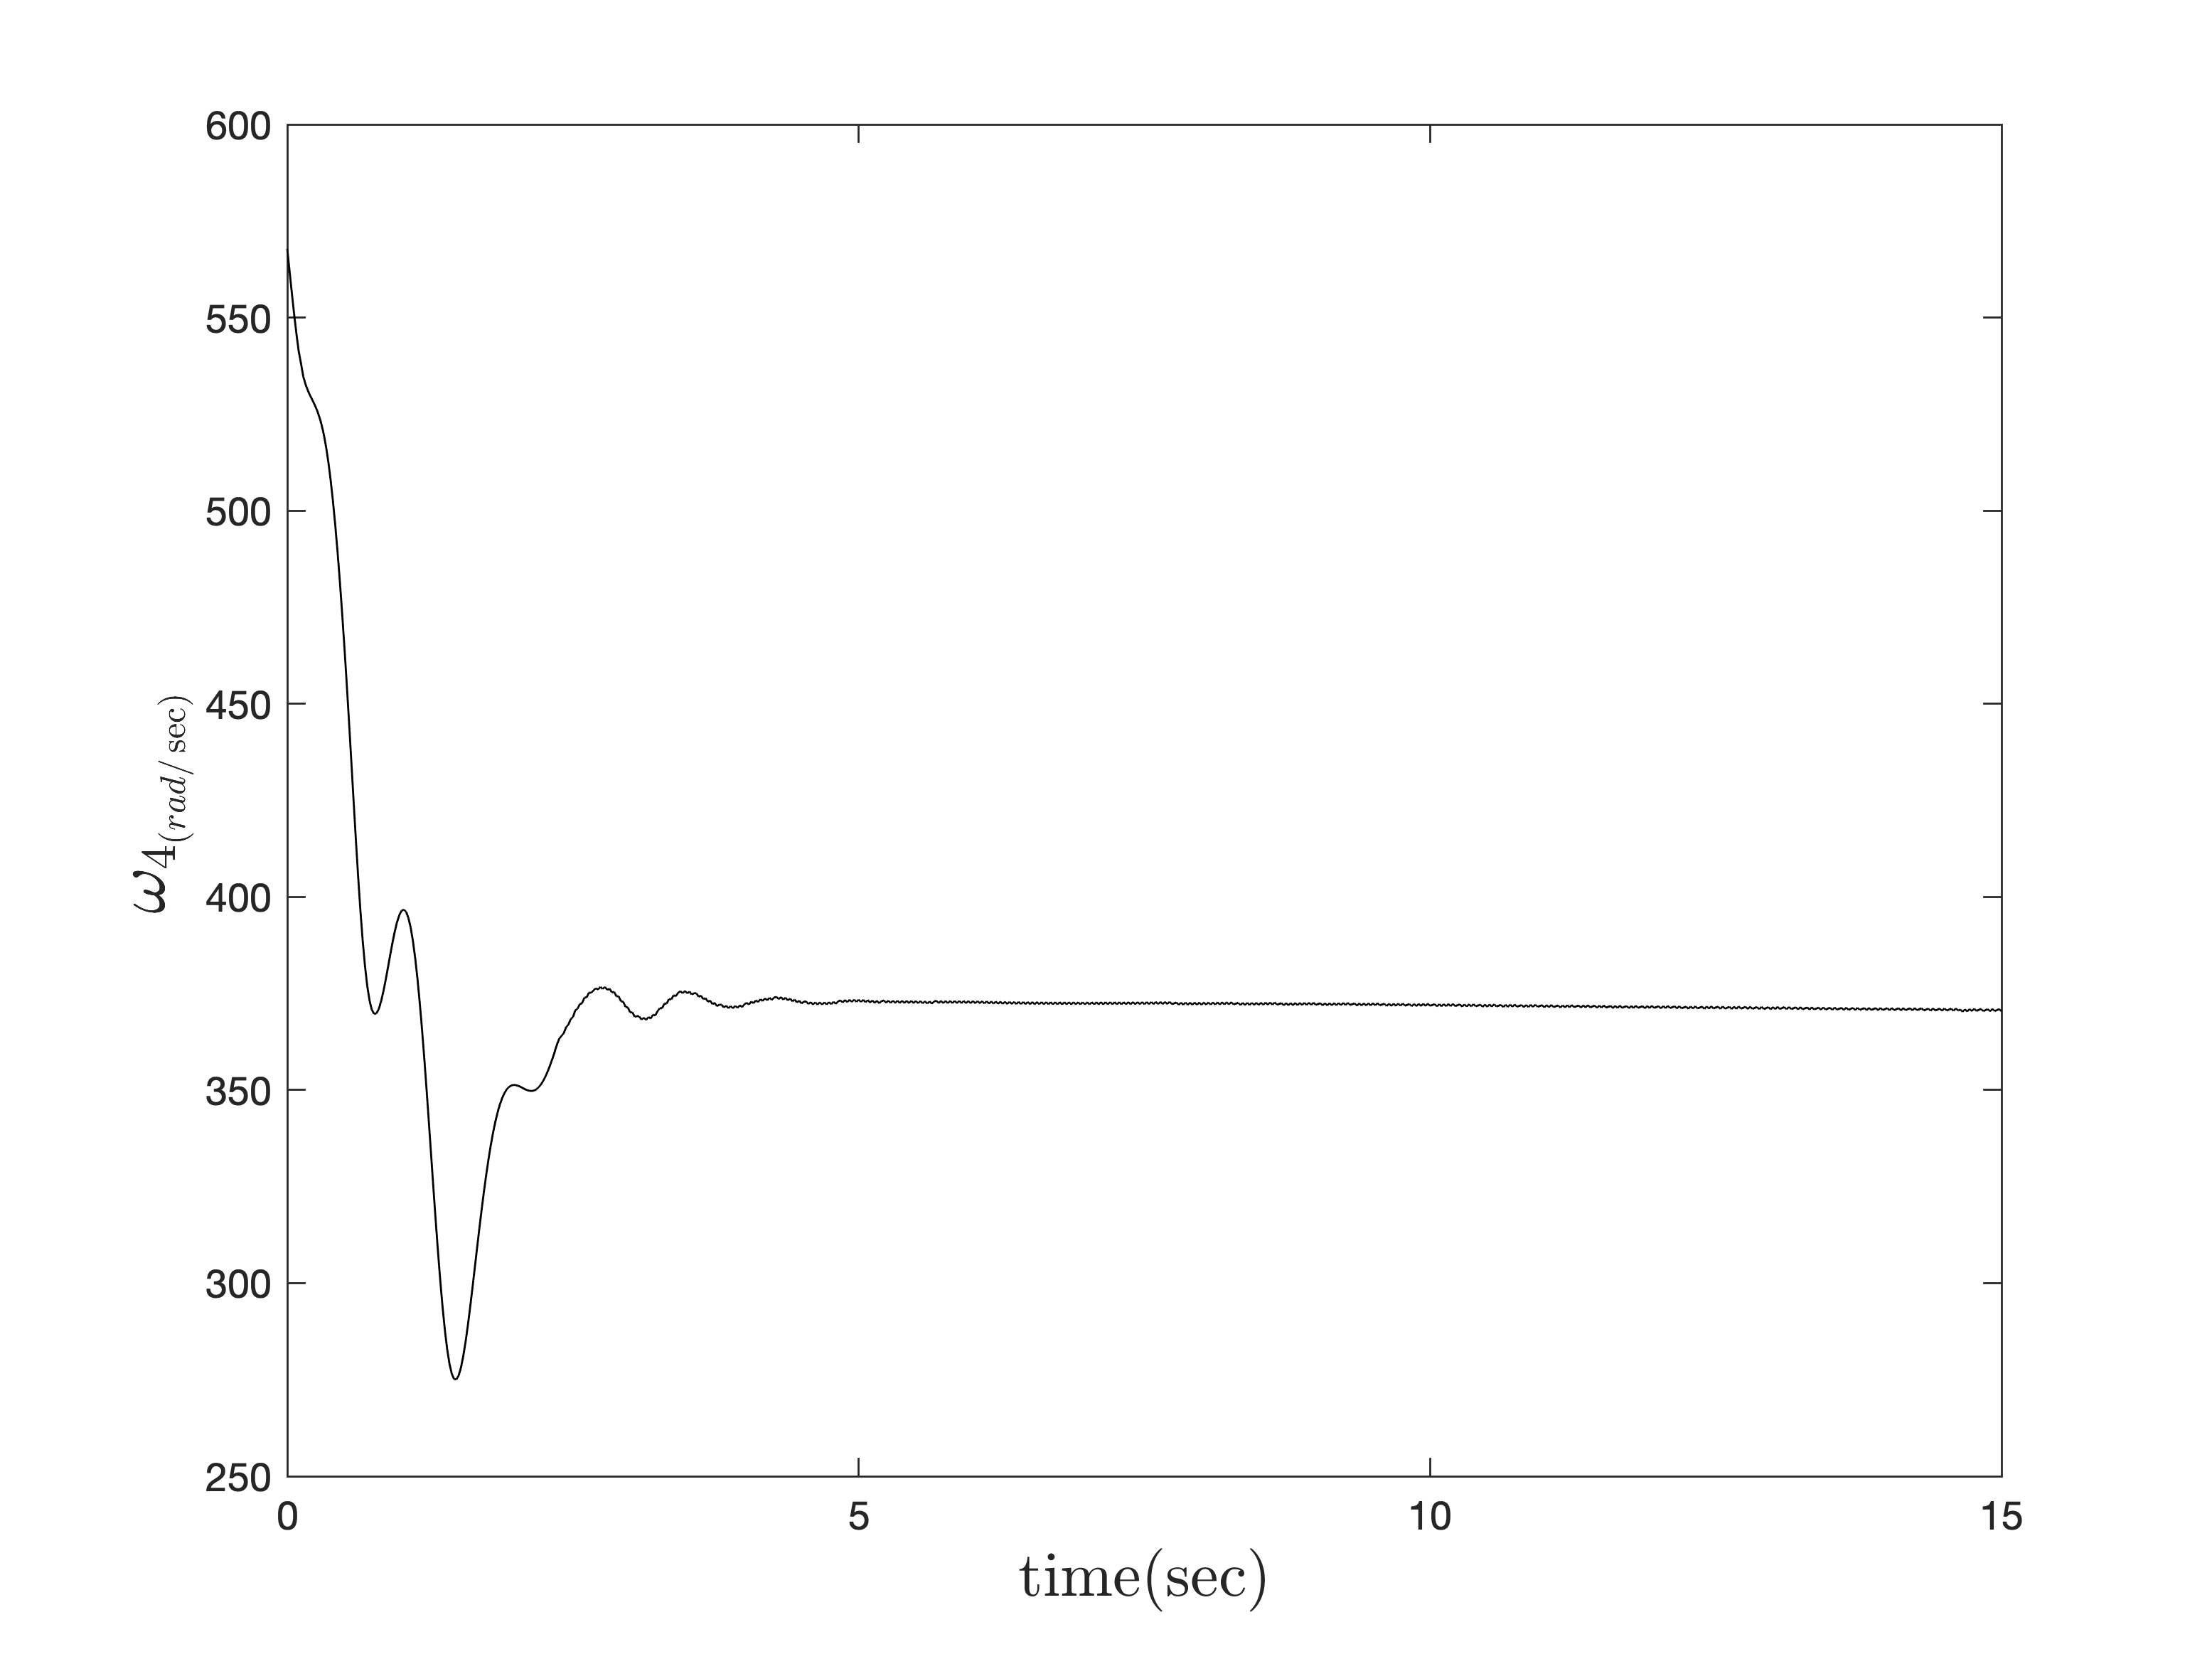
\includegraphics[width=.45\linewidth]{../Figures/MIL/LQIDG/3DOF/lqidg_roll_pitch_Omega_4_nn.png}
	}
	\caption{‫‪فرمان کنترلی موتورها در کنترل وضعیت (تعقیب ورودی صفر)}
\end{figure}

\subsubsection{شبیه‌سازی کنترل‌کننده به‌صورت چهار ورودی}\label{mimo_sim}
\setcounter{MaxMatrixCols}{20}

\begin{equation}
	\begin{split}
		\boldsymbol{K_{a_{1_{roll}}}} &= \begin{bmatrix}
258228.43 & 0.00 & 0.00 & 0.00 \\ 
0.00 & 33152686.22 & 0.00 & 0.00 \\ 
0.00 & 0.00 & 160.15 & 0.00 \\ 
0.00 & 0.00 & 0.00 & 7541.49 \\ 
		\end{bmatrix}\\
	 \boldsymbol{K_{a_{1_{pitch}}}} & = \begin{bmatrix}
382.64 & 0.00 & 0.00 & 0.00 \\ 
0.00 & 20246.38 & 0.00 & 0.00 \\ 
0.00 & 0.00 & 2472592.13 & 0.00 \\ 
0.00 & 0.00 & 0.00 & 60676037.12 \\ 
\end{bmatrix}\\
		\boldsymbol{K_{a_{1_{yaw}}}} &= 
		\begin{bmatrix}
3390219.36 & 0.00 & 0.00 & 0.00 \\ 
0.00 & 45.04 & 0.00 & 0.00 \\ 
0.00 & 0.00 & 41049.01 & 0.00 \\ 
0.00 & 0.00 & 0.00 & 881966.56 \\ 
		\end{bmatrix}
	\end{split}
\end{equation}


\begin{equation}
	\boldsymbol{Q_{a_{LQIDG}}}  = 
	\begin{bmatrix}
		\boldsymbol{K_{a_{1_{roll}}}}  & 0 & 0\\
		0 & \boldsymbol{K_{a_{1_{pitch}}}} & 0\\
		0 & 0 & \boldsymbol{K_{a_{1_{yaw}}}}
	\end{bmatrix}, \quad  \boldsymbol{R_{1_{LQDG}}} = 1, \boldsymbol{R_{2_{LQDG}}} = 15.1793
\end{equation}

در گام بعد، با حل معادله
(\ref{coupled_riccatti_LQIDG})
(برای سادگی ماتریس‌های وزنی $\boldsymbol{{Q}_{a_2}}$ و $\boldsymbol{{Q}_{a_1}}$مساوی در نظر گرفته شده‌است)
ماتریس
$\boldsymbol{{K}_1}$ به دست می‌آید.
در نهایت فرمان کنترلی بهینه بازیکن اول از رابطه
(\ref{LQIDG_u})
به دست می‌آید (به علت حجم زیاد ماتریس‌ها از آوردن مستقیم آنها پرهیز شده‌است).

%\begin{equation*}
%	\boldsymbol{Q_{a_{LQIDG}}} = 
%	\begin{bmatrix}
%		631.85 & 0.00 & 0.00 & 0.00 & 0.00 & 0.00 & 0.00 & 0.00 & 0.00 & 0.00 & 0.00 & 0.00\\ 
%		0.00 & 214.28 & 0.00 & 0.00 & 0.00 & 0.00 & 0.00 & 0.00 & 0.00 & 0.00 & 0.00 & 0.00\\ 
%		0.00 & 0.00 & 7.91 & 0.00 & 0.00 & 0.00 & 0.00 & 0.00 & 0.00 & 0.00 & 0.00 & 0.00\\ 
%		0.00 & 0.00 & 0.00 & 0.01 & 0.00 & 0.00 & 0.00 & 0.00 & 0.00 & 0.00 & 0.00 & 0.00\\ 
%		0.00 & 0.00 & 0.00 & 0.00 & 0.01 & 0.00 & 0.00 & 0.00 & 0.00 & 0.00 & 0.00 & 0.00\\ 
%		0.00 & 0.00 & 0.00 & 0.00 & 0.00 & 873.93 & 0.00 & 0.00 & 0.00 & 0.00 & 0.00 & 0.00\\ 
%		0.00 & 0.00 & 0.00 & 0.00 & 0.00 & 0.00 & 9853.09 & 0.00 & 0.00 & 0.00 & 0.00 & 0.00\\ 
%		0.00 & 0.00 & 0.00 & 0.00 & 0.00 & 0.00 & 0.00 & 0.12 & 0.00 & 0.00 & 0.00 & 0.00\\ 
%		0.00 & 0.00 & 0.00 & 0.00 & 0.00 & 0.00 & 0.00 & 0.00 & 0.00 & 0.00 & 0.00 & 0.00\\ 
%		0.00 & 0.00 & 0.00 & 0.00 & 0.00 & 0.00 & 0.00 & 0.00 & 0.00 & 0.00 & 0.00 & 0.00\\ 
%		0.00 & 0.00 & 0.00 & 0.00 & 0.00 & 0.00 & 0.00 & 0.00 & 0.00 & 0.00 & 0.00 & 0.00\\ 
%		0.00 & 0.00 & 0.00 & 0.00 & 0.00 & 0.00 & 0.00 & 0.00 & 0.00 & 0.00 & 0.00 & 3.33\\ 
%		
%	\end{bmatrix}
%\end{equation*}
%
%\begin{equation*}
%	\begin{bmatrix}
%		-0.00 & 101.23 & 5.33 & -0.00 & 48.29 & 45.40 & 0.00 & 0.07 & 0.34 & -0.00 & -0.00 & 0.15\\ 
%		241.81 & -0.00 & -5.33 & 86.14 & -0.00 & -45.40 & 57.31 & 0.00 & -0.34 & 0.00 & -0.00 & -0.15\\ 
%		-0.00 & -101.23 & 5.33 & -0.00 & -48.29 & 45.40 & 0.00 & -0.07 & 0.34 & -0.00 & 0.00 & 0.15\\ 
%		-241.81 & -0.00 & -5.33 & -86.14 & -0.00 & -45.40 & -57.31 & 0.00 & -0.34 & -0.00 & -0.00 & -0.15\\ 
%	\end{bmatrix}
%\end{equation*}
%
%
%\begin{equation*}
%	\boldsymbol{K_{a_1}} = 
%	\begin{bmatrix}
%34004 & -0 & -0 & 11130 & -0 & -0 & 14810 & 0 & -0 & -9 & -0 & -0\\ 
%-0 & 7396 & 0 & -0 & 3498 & 0 & 0 & 11 & 0 & -0 & -10 & 0\\ 
%-0 & 0 & 1504 & -0 & 0 & 10019 & 0 & -0 & 95 & -0 & 0 & -27\\ 
%11129 & -0 & -0 & 3965 & -0 & -0 & 2638 & 0 & -0 & 0 & -0 & -0\\ 
%-0 & 3498 & 0 & -0 & 1669 & 0 & 0 & 3 & 0 & -0 & -0 & 0\\ 
%-0 & 0 & 10019 & -0 & 0 & 85406 & 0 & -0 & 630 & -0 & 0 & 277\\ 
%14810 & 0 & 0 & 2638 & 0 & 0 & 24372 & -0 & 0 & -0 & 0 & 0\\ 
%0 & 11 & -0 & 0 & 3 & -0 & -0 & 11 & -0 & 0 & -0 & -0\\ 
%-0 & 0 & 95 & -0 & 0 & 630 & 0 & -0 & 7 & -0 & 0 & -2\\ 
%-10 & -0 & -0 & -0 & -0 & -0 & -0 & 0 & -0 & 10 & -0 & -0\\ 
%-0 & -10 & 0 & -0 & -0 & 0 & 0 & -0 & 0 & -0 & 9 & 0\\ 
%-0 & 0 & -27 & -0 & 0 & 277 & 0 & -0 & -2 & -0 & 0 & 59\\ 
%
%	\end{bmatrix}
%\end{equation*}



\begin{figure}[H]
	\centering
	\subfigure[تغییرات زاویه رول]{
		\centering
		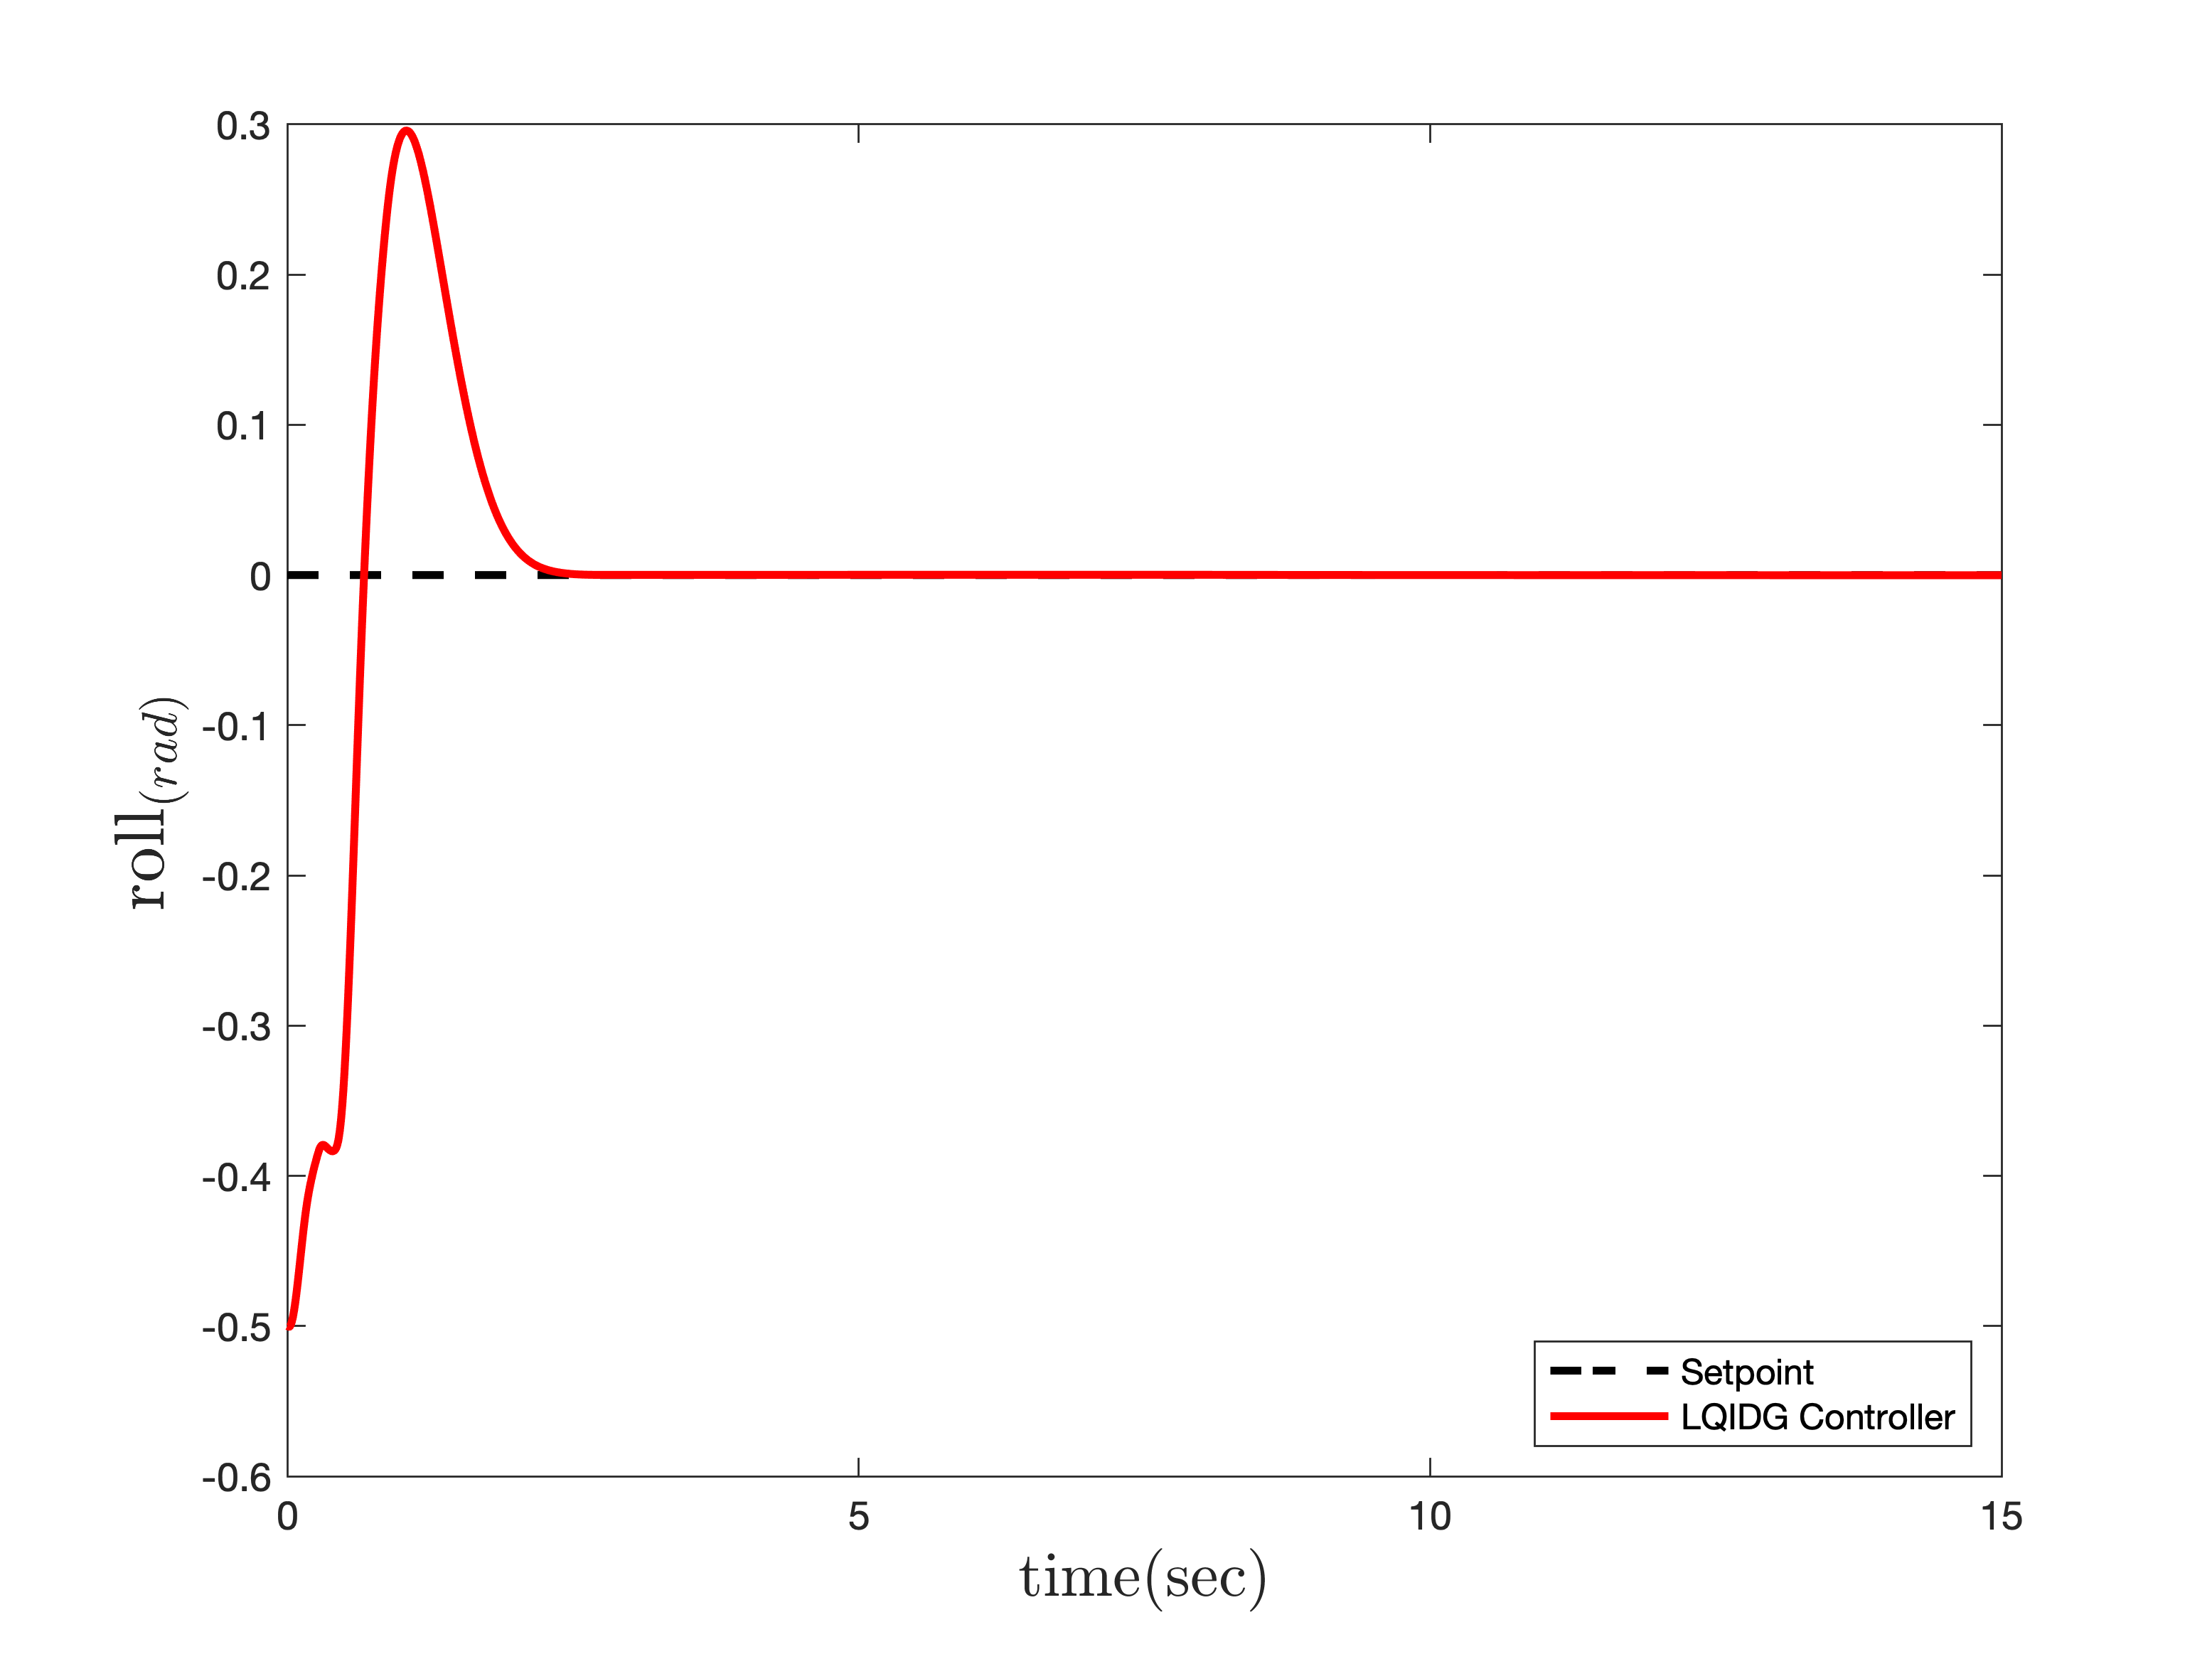
\includegraphics[width=.48\linewidth]{../Figures/MIL/LQIDG/MIMO/lqidg_roll_nn.png}
	}
	\subfigure[تغییرات زاویه پیچ]{
		\centering
		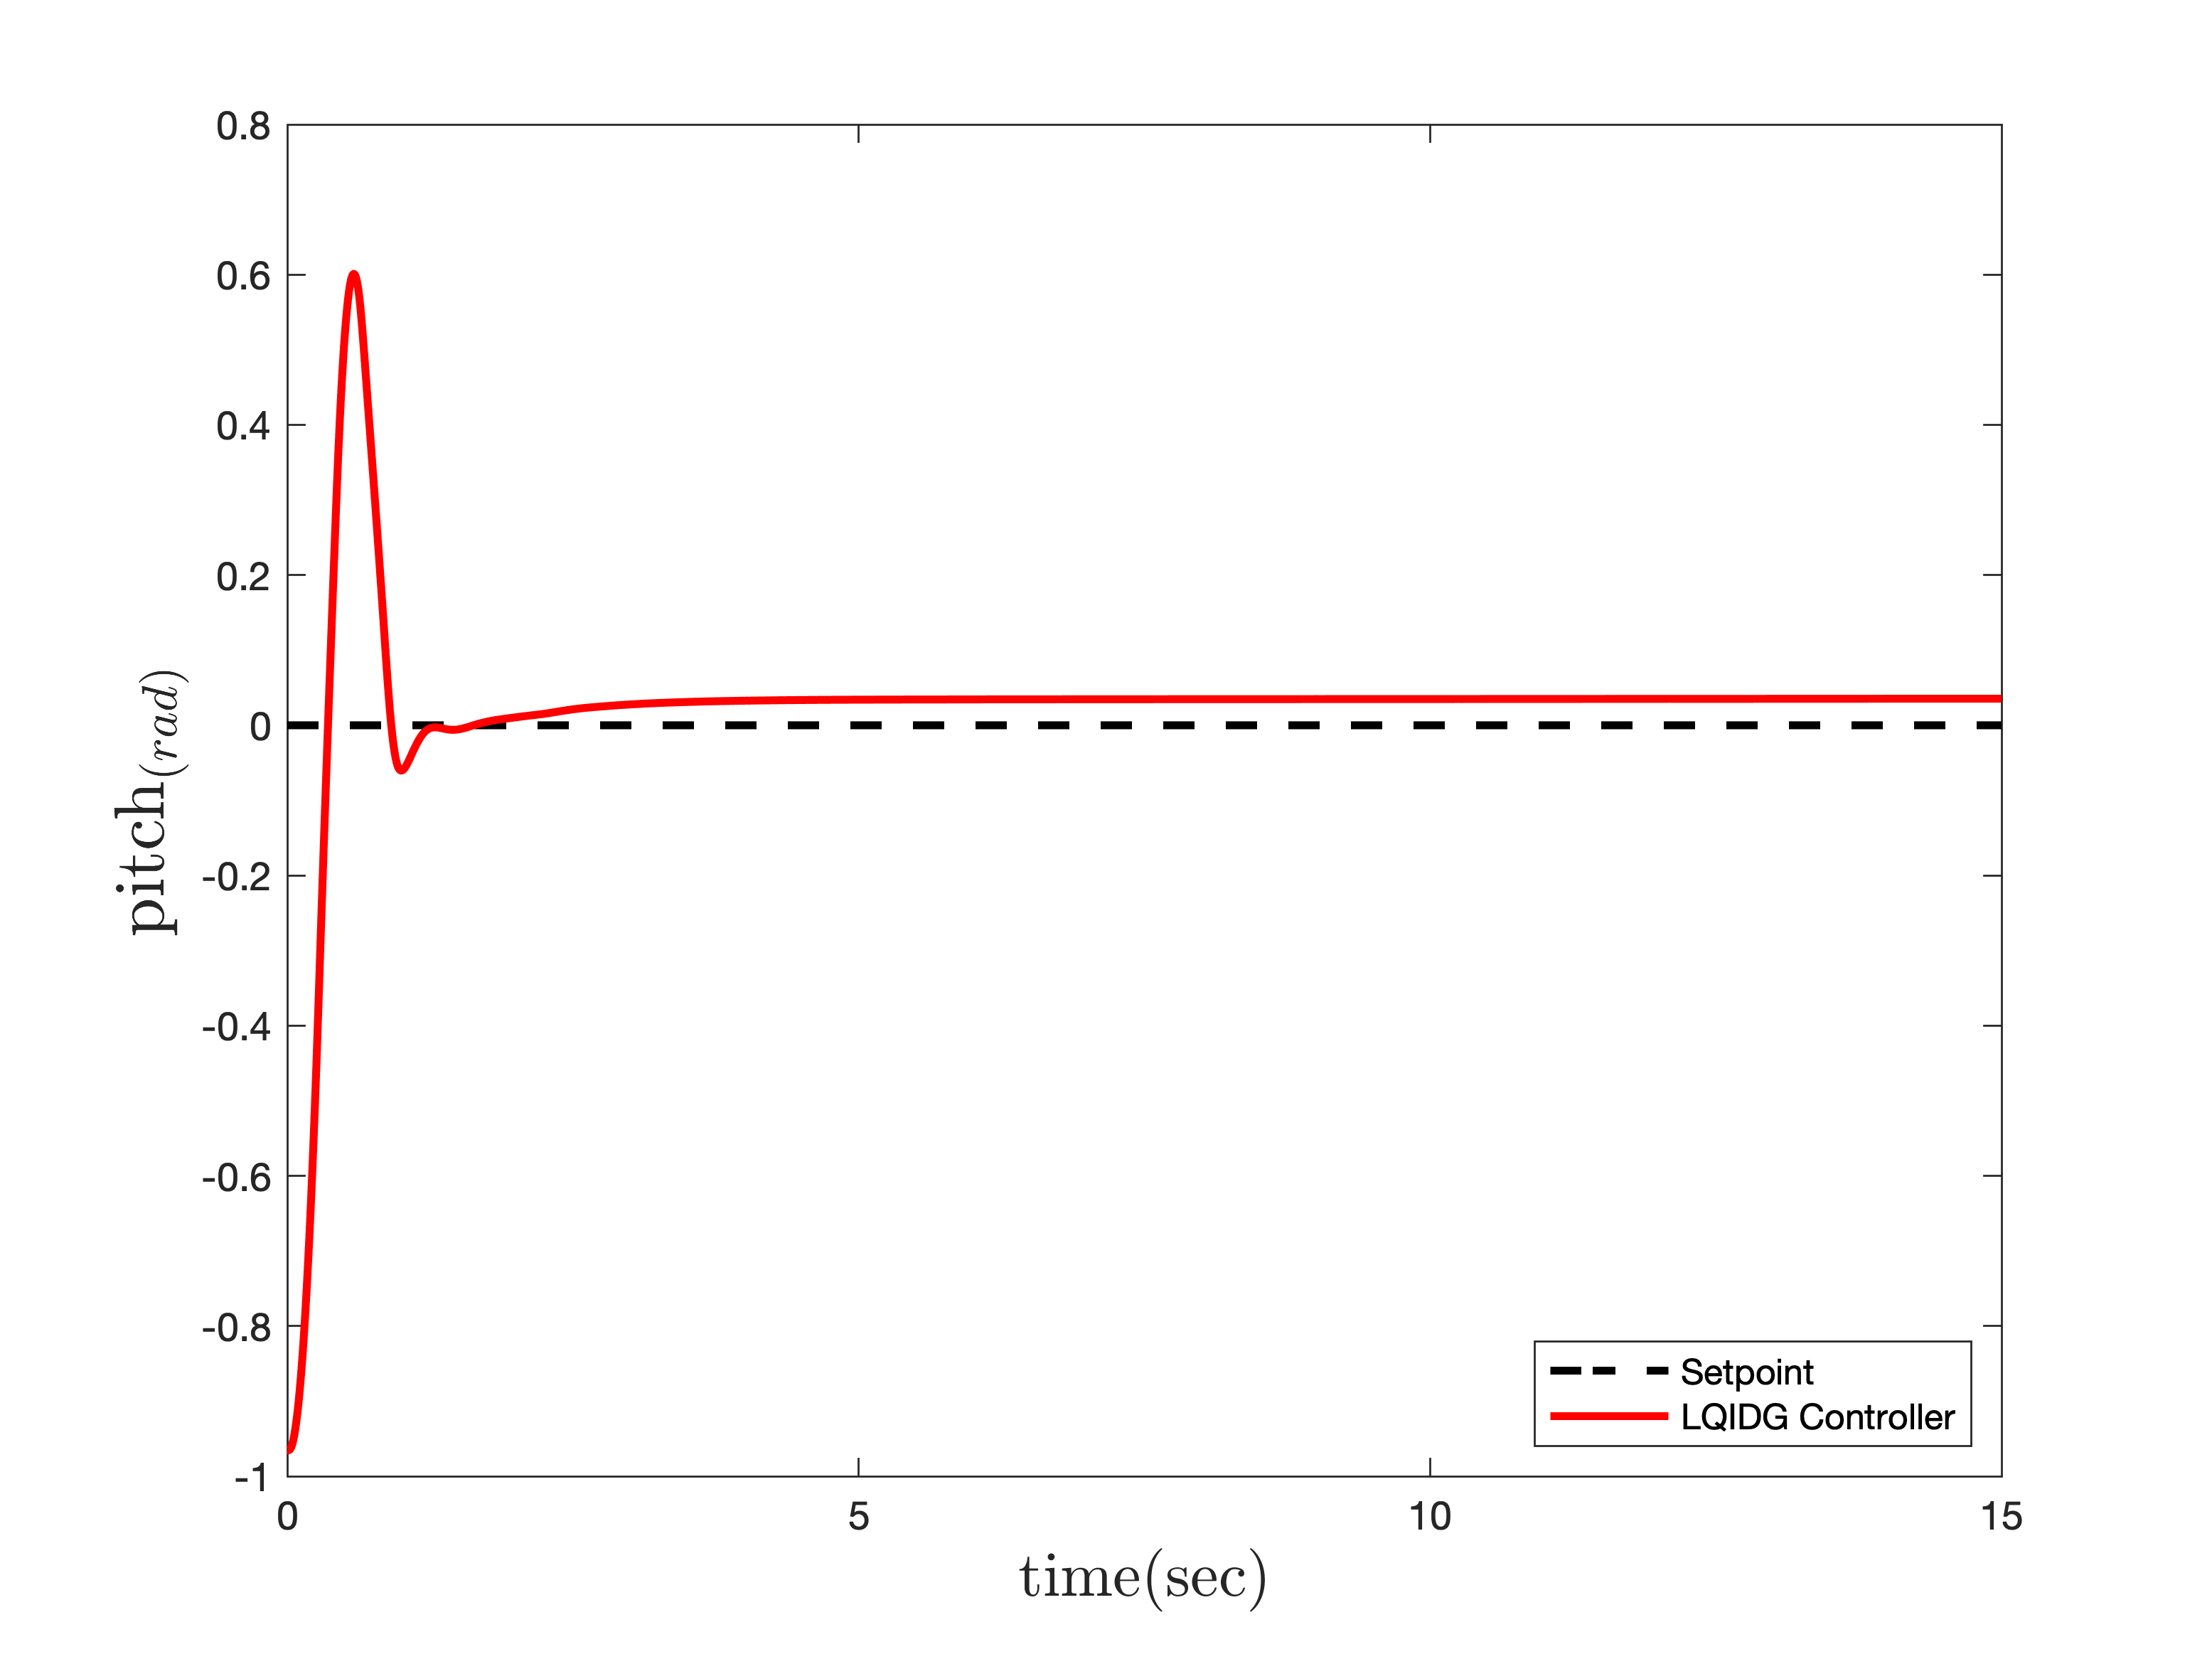
\includegraphics[width=.48\linewidth]{../Figures/MIL/LQIDG/MIMO/lqidg_pitch_nn.png}
	}
	\subfigure[تغییرات زاویه یاو]{
		\centering
		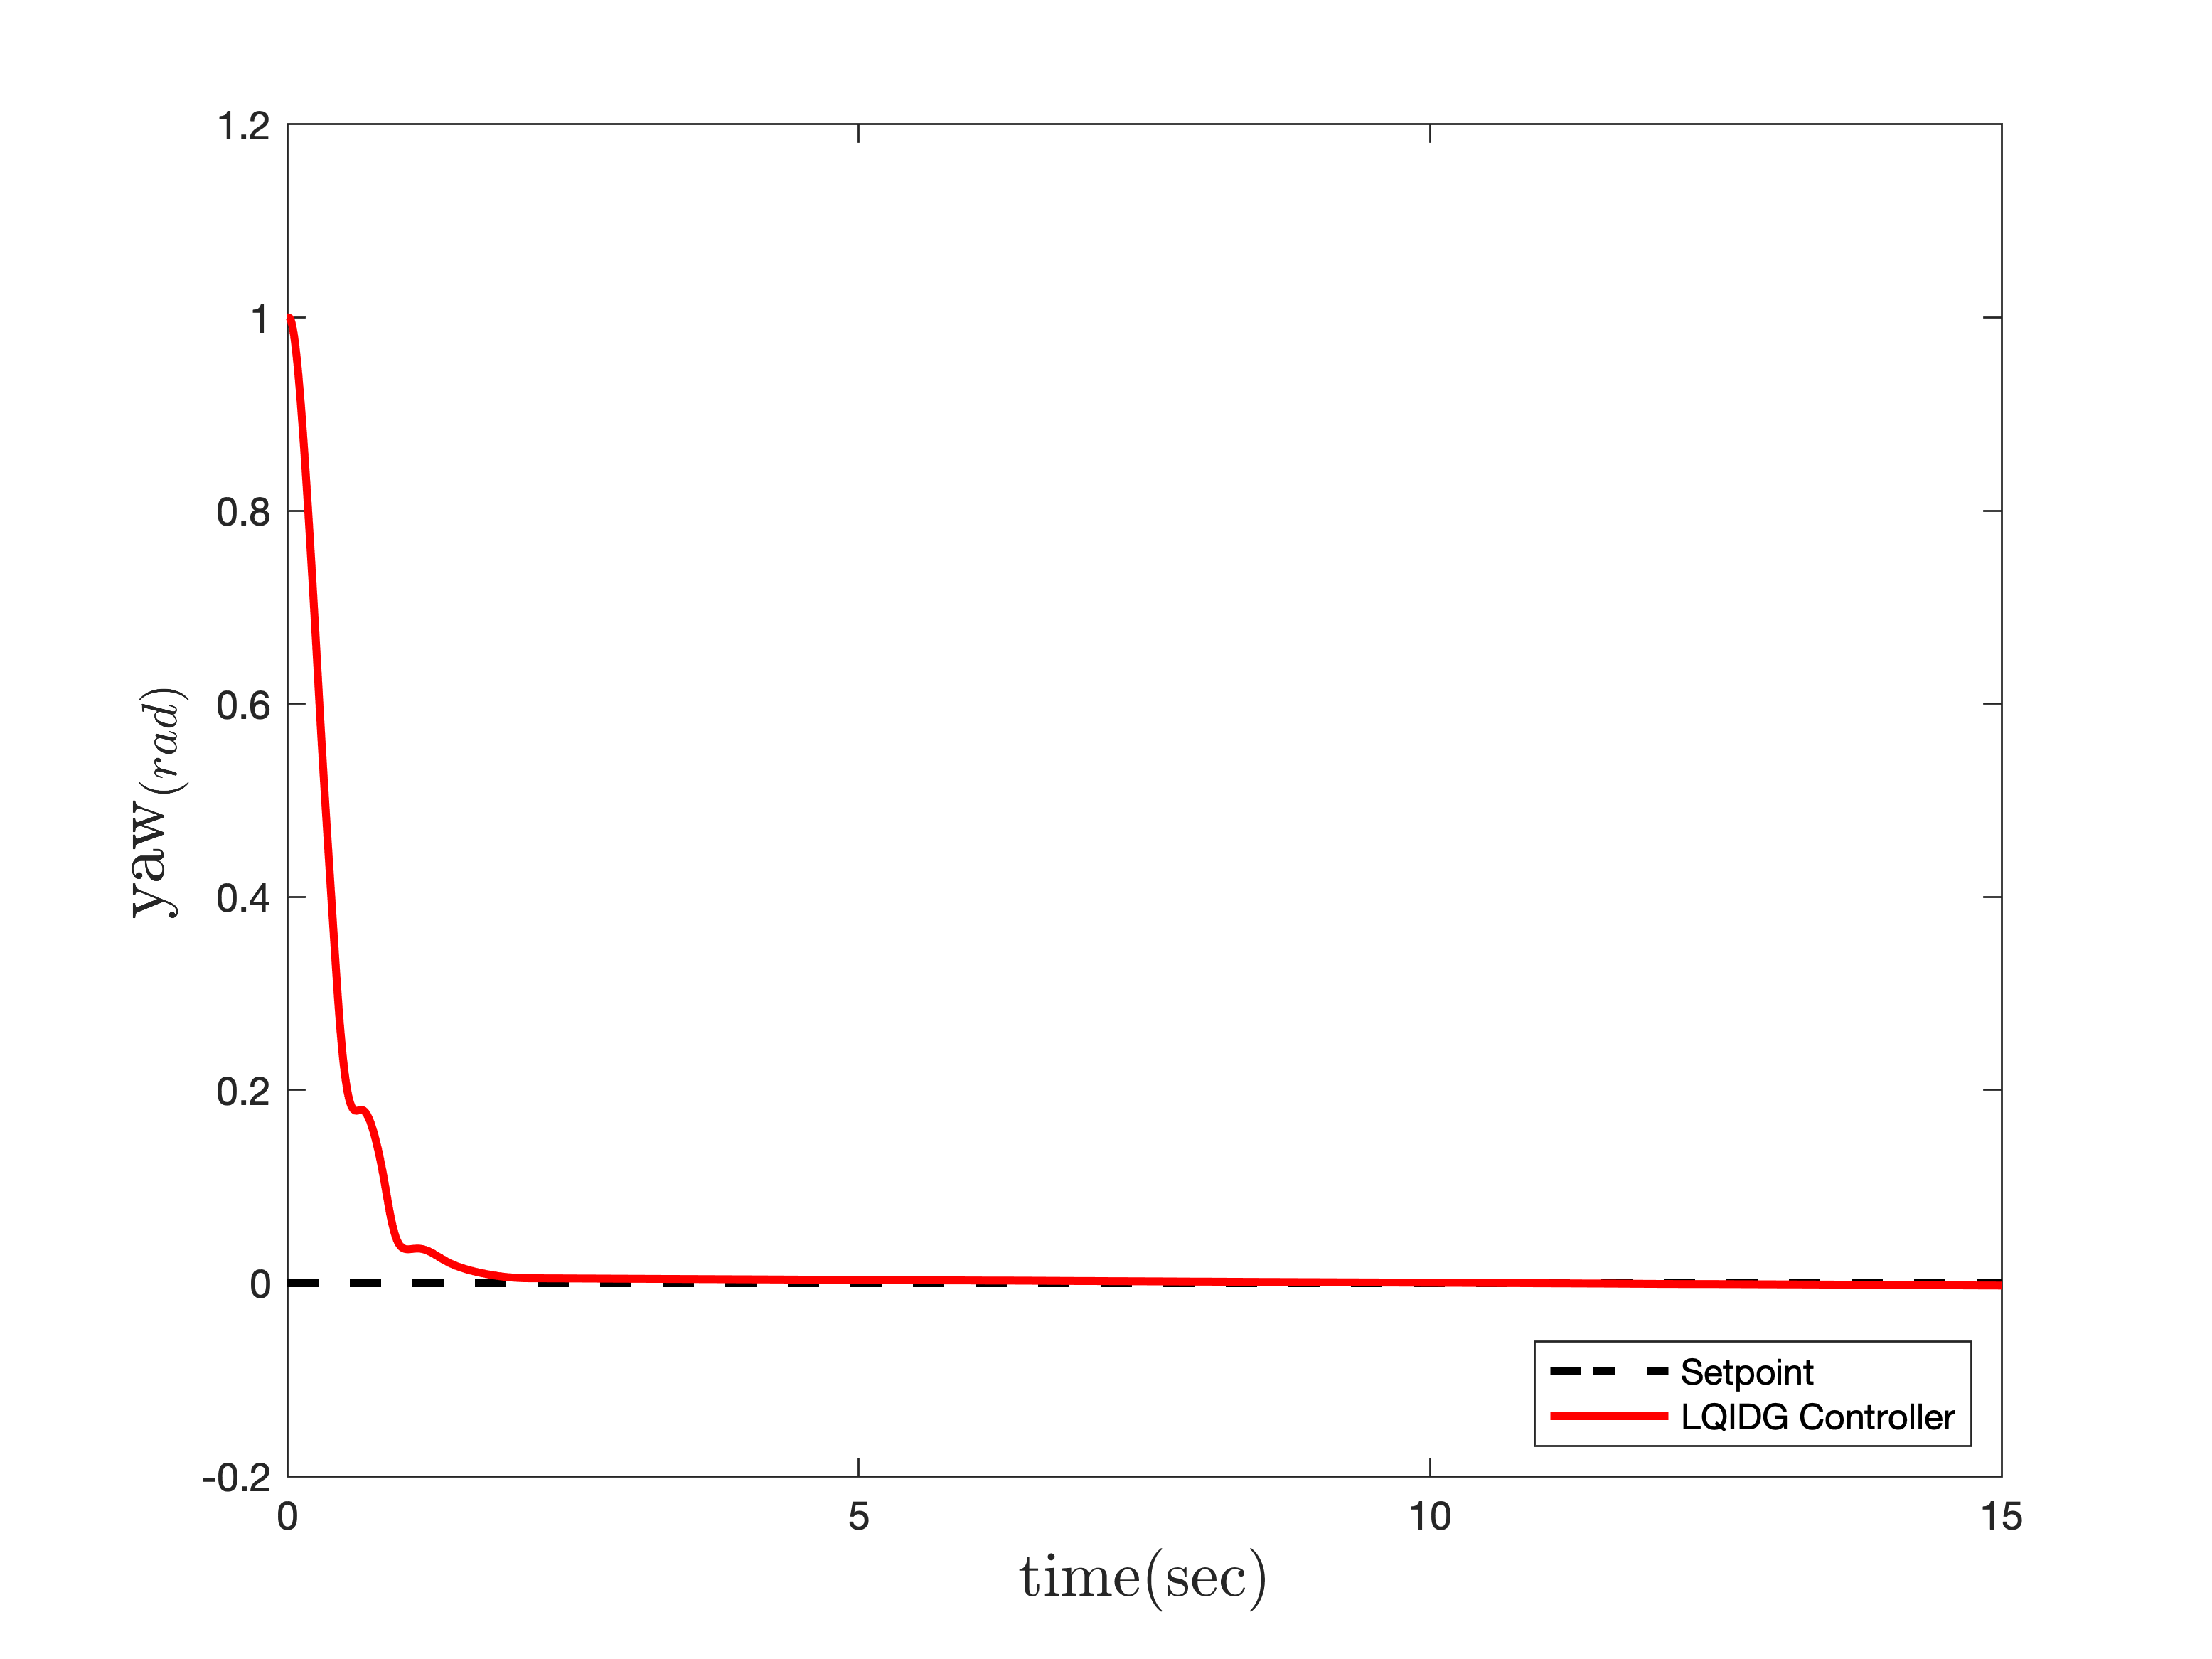
\includegraphics[width=.48\linewidth]{../Figures/MIL/LQIDG/MIMO/lqidg_yaw_nn.png}
	}
	\caption{‫‪عملکرد کنترل‌کننده \lr{LQIDG} در کنترل وضعیت (تعقیب ورودی صفر)}
	\label{lqidg_roll_pitch_yaw_fig_simulation_MIMO}
\end{figure}


\begin{figure}[H]
	\centering
	\subfigure[موتور شماره یک]{
		\centering
		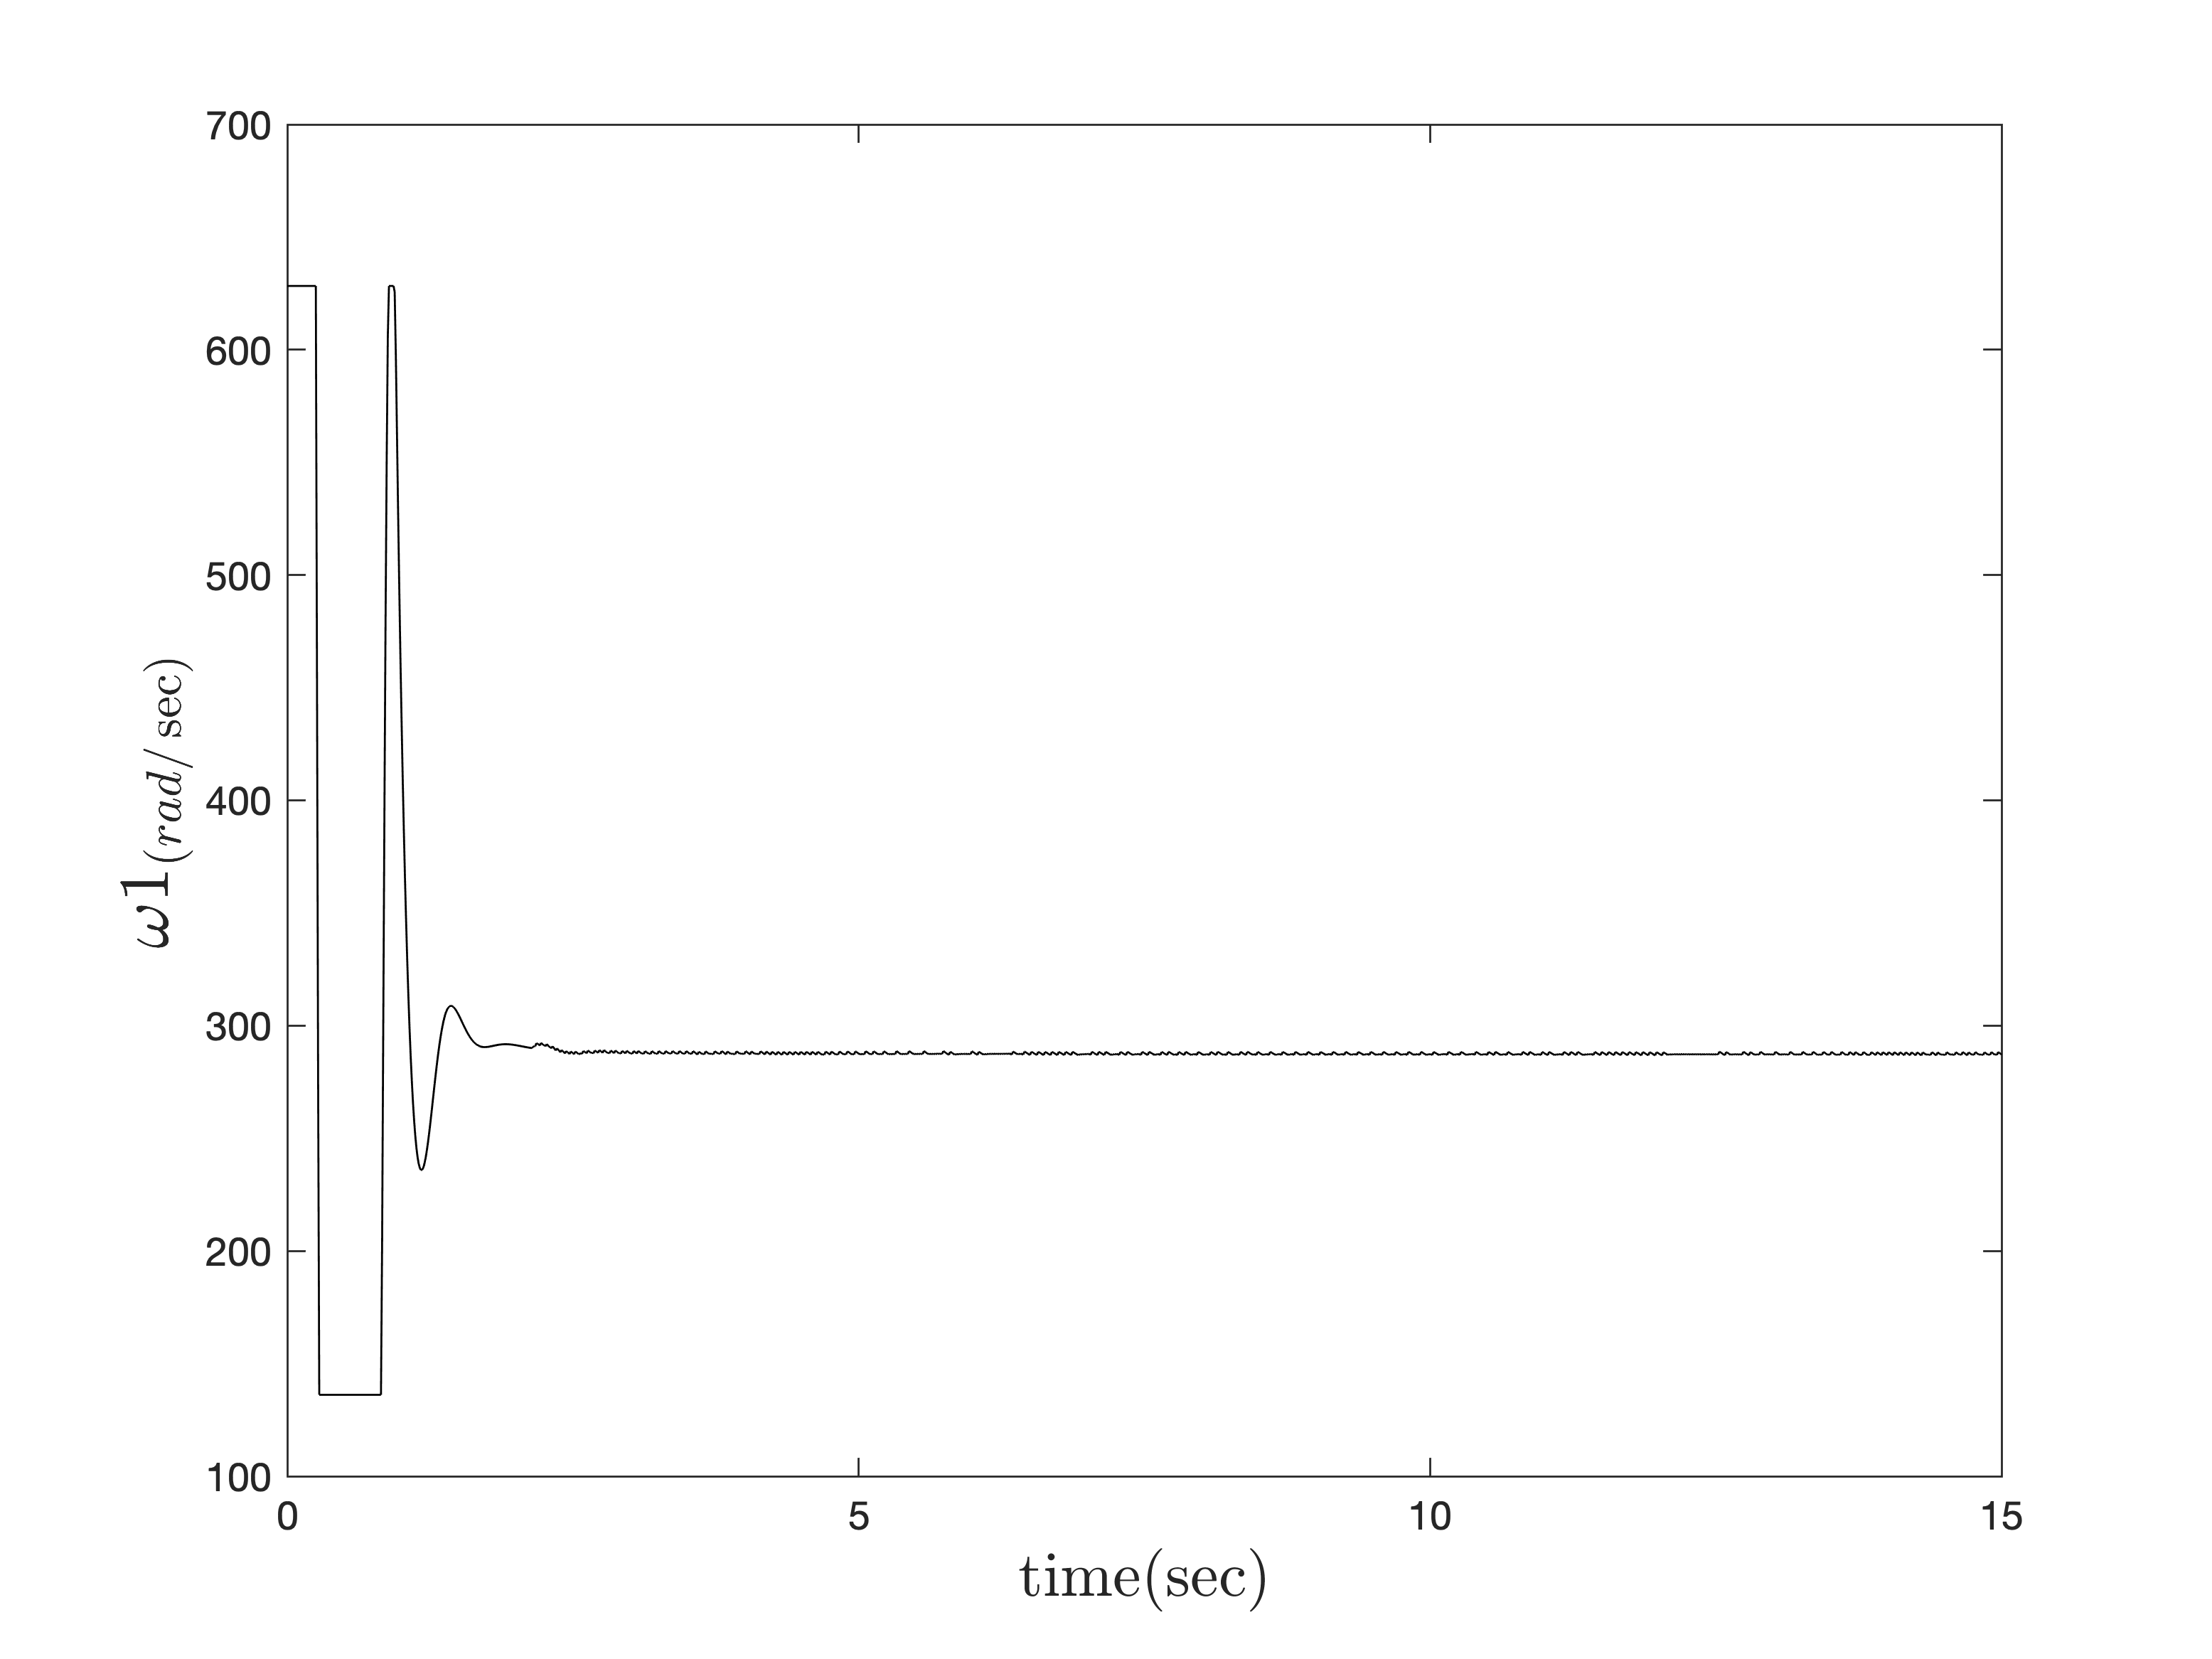
\includegraphics[width=.45\linewidth]{../Figures/MIL/LQIDG/MIMO/lqidg_roll_pitch_Omega1_nn.png}
	}
	\subfigure[موتور شماره دو]{
		\centering
		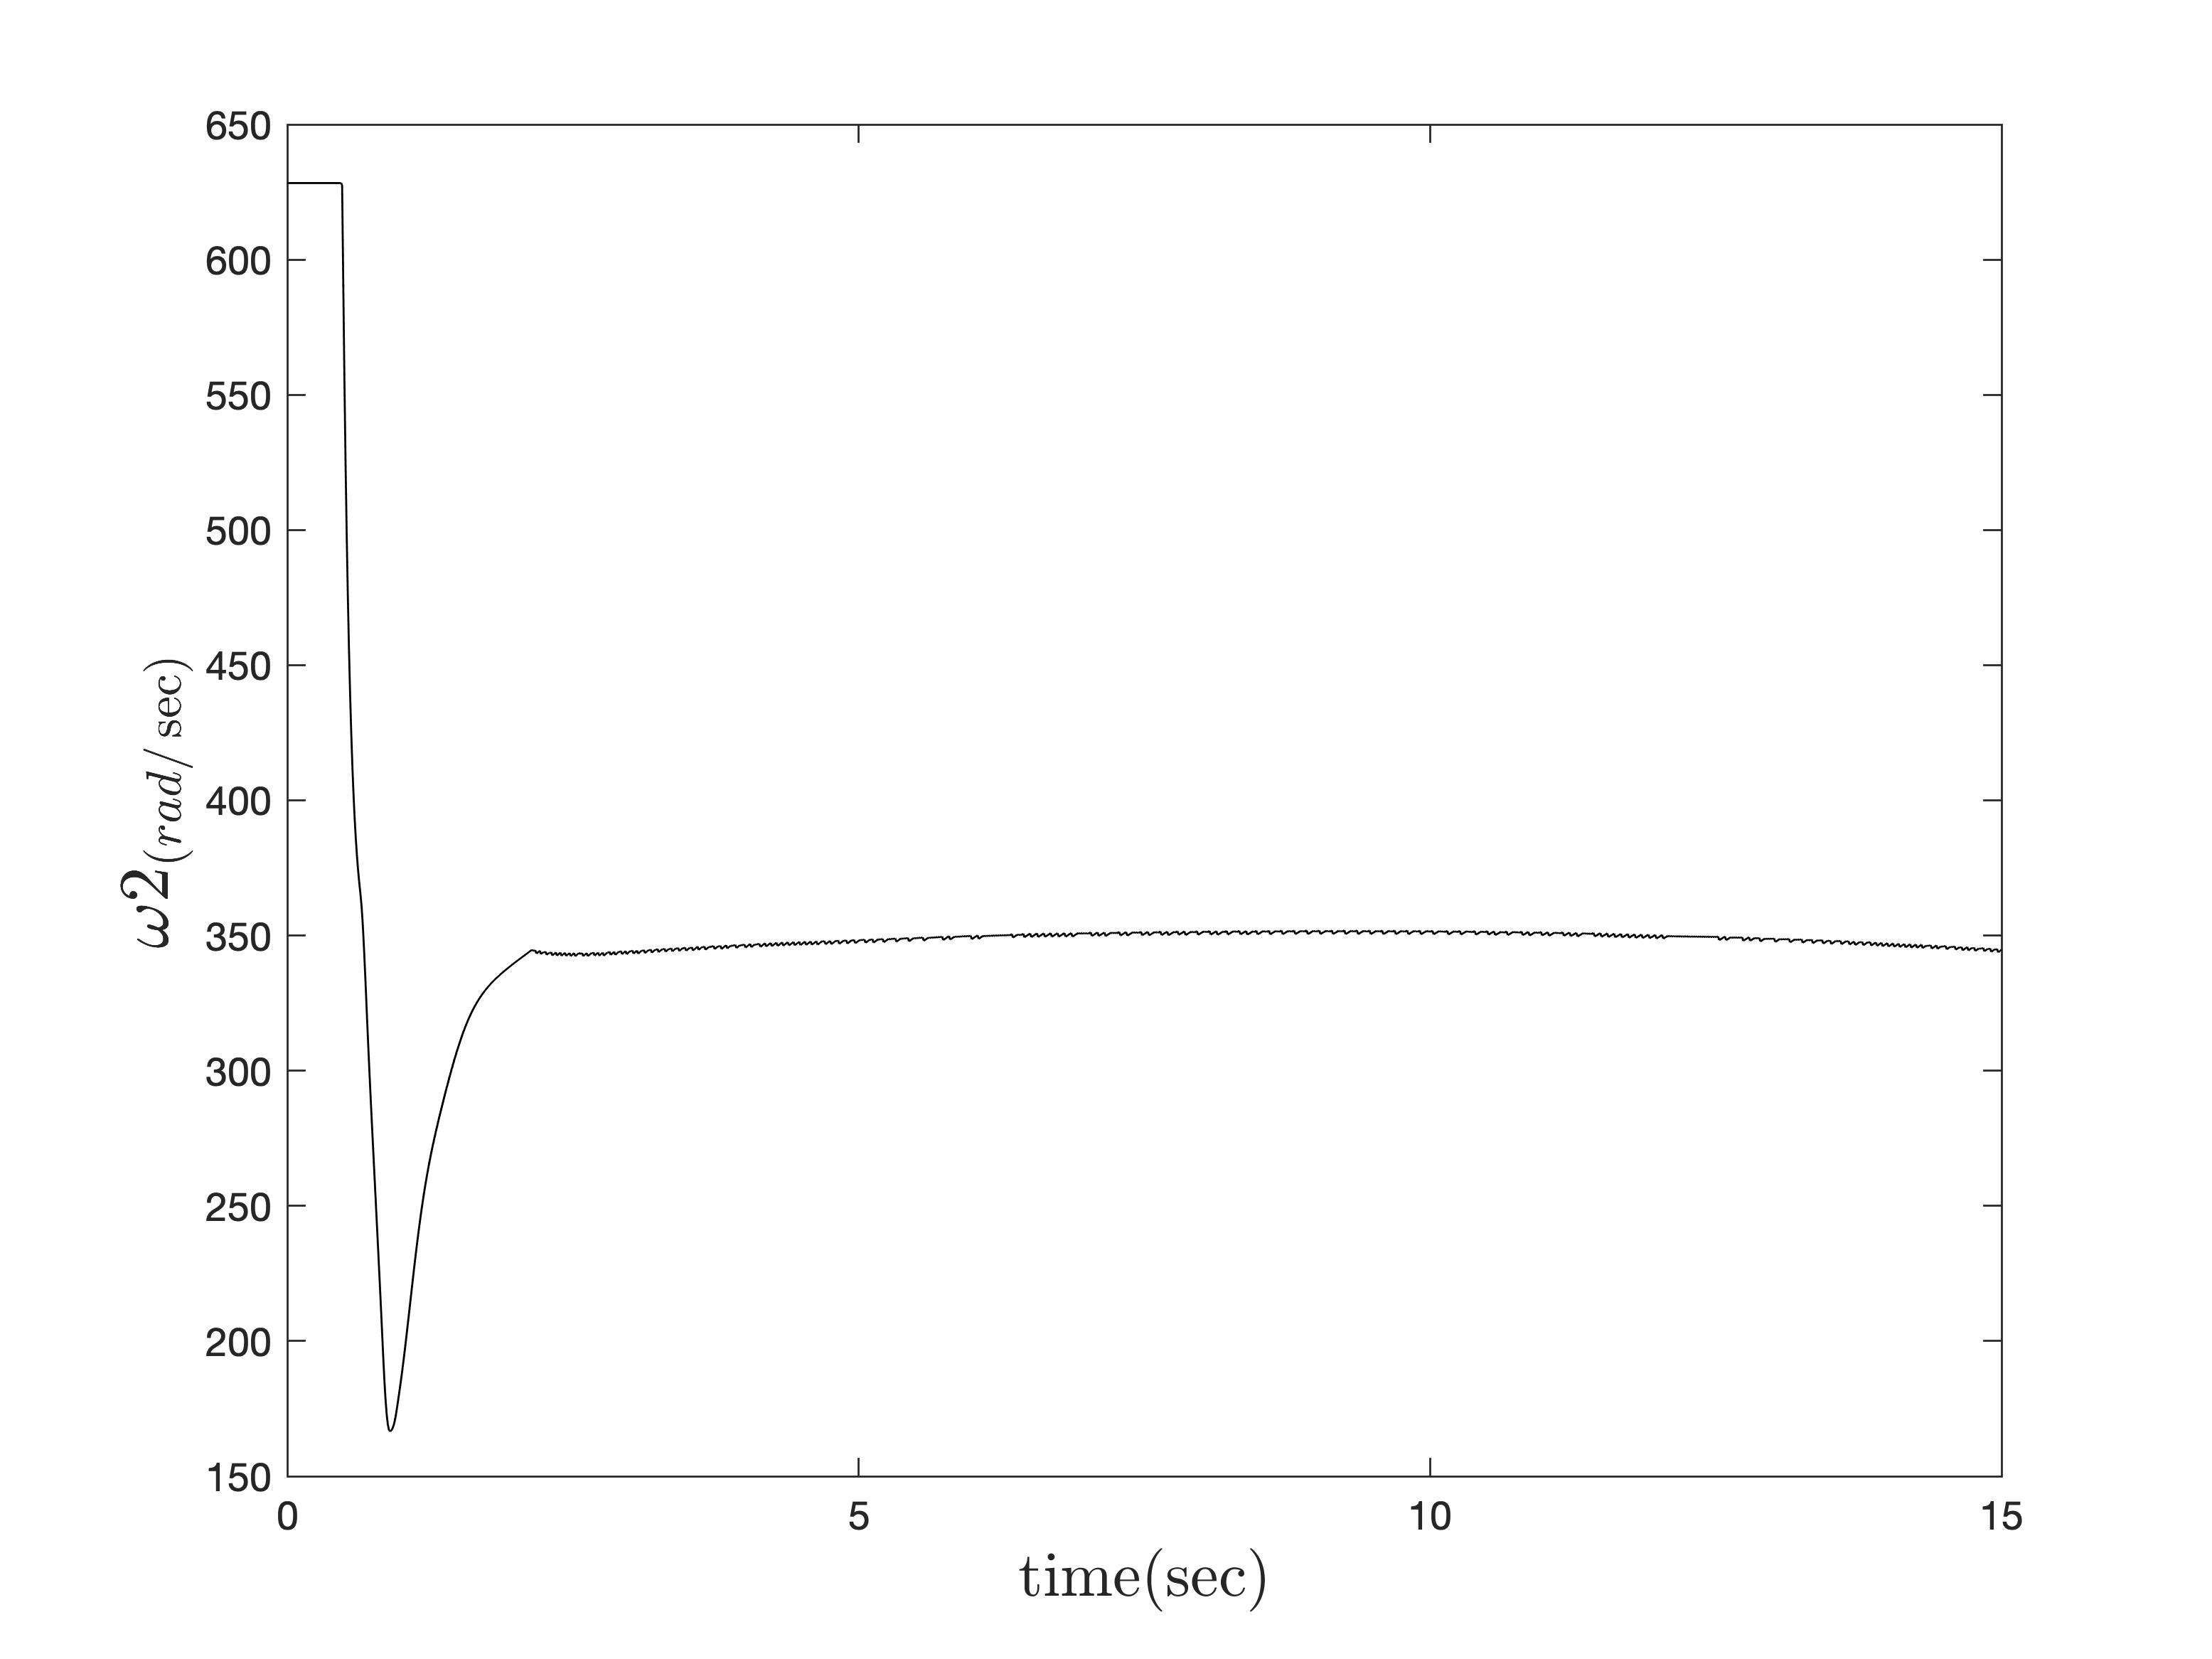
\includegraphics[width=.45\linewidth]{../Figures/MIL/LQIDG/MIMO/lqidg_roll_pitch_Omega2_nn.png}
	}
	\subfigure[موتور شماره سه]{
		\centering
		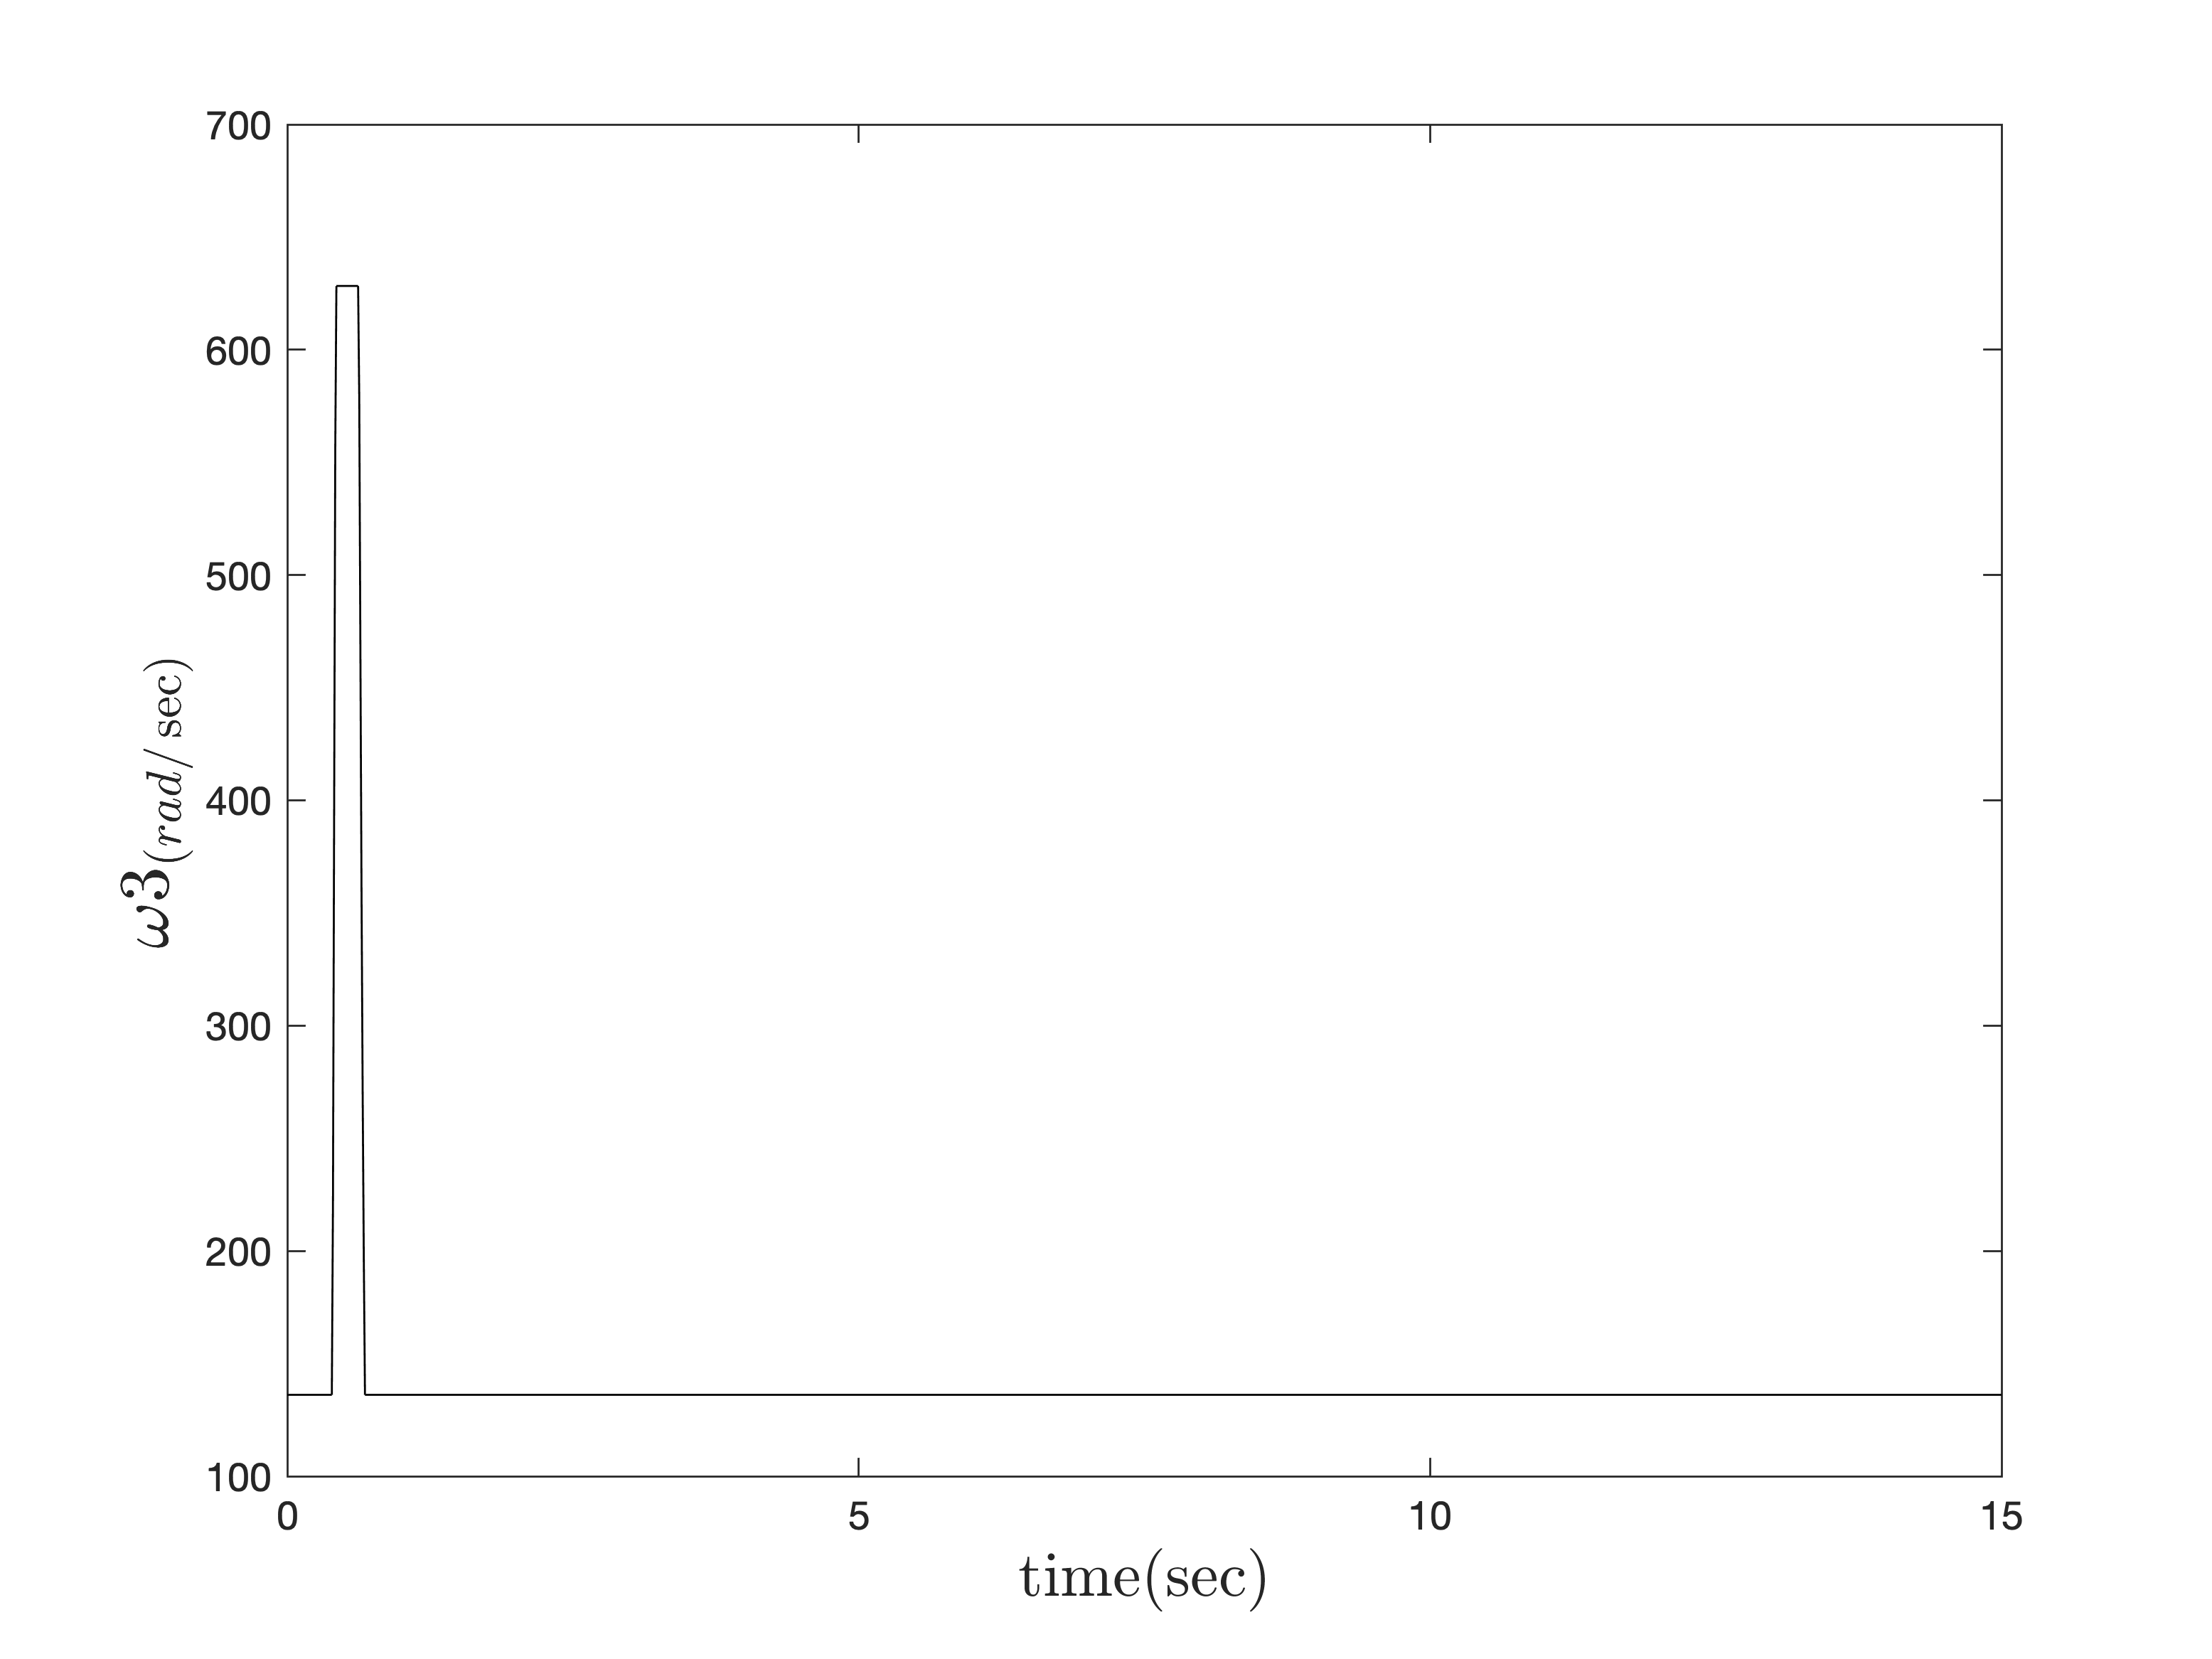
\includegraphics[width=.45\linewidth]{../Figures/MIL/LQIDG/MIMO/lqidg_roll_pitch_Omega3_nn.png}
	}
	\subfigure[موتور شماره چهار]{
		\centering
		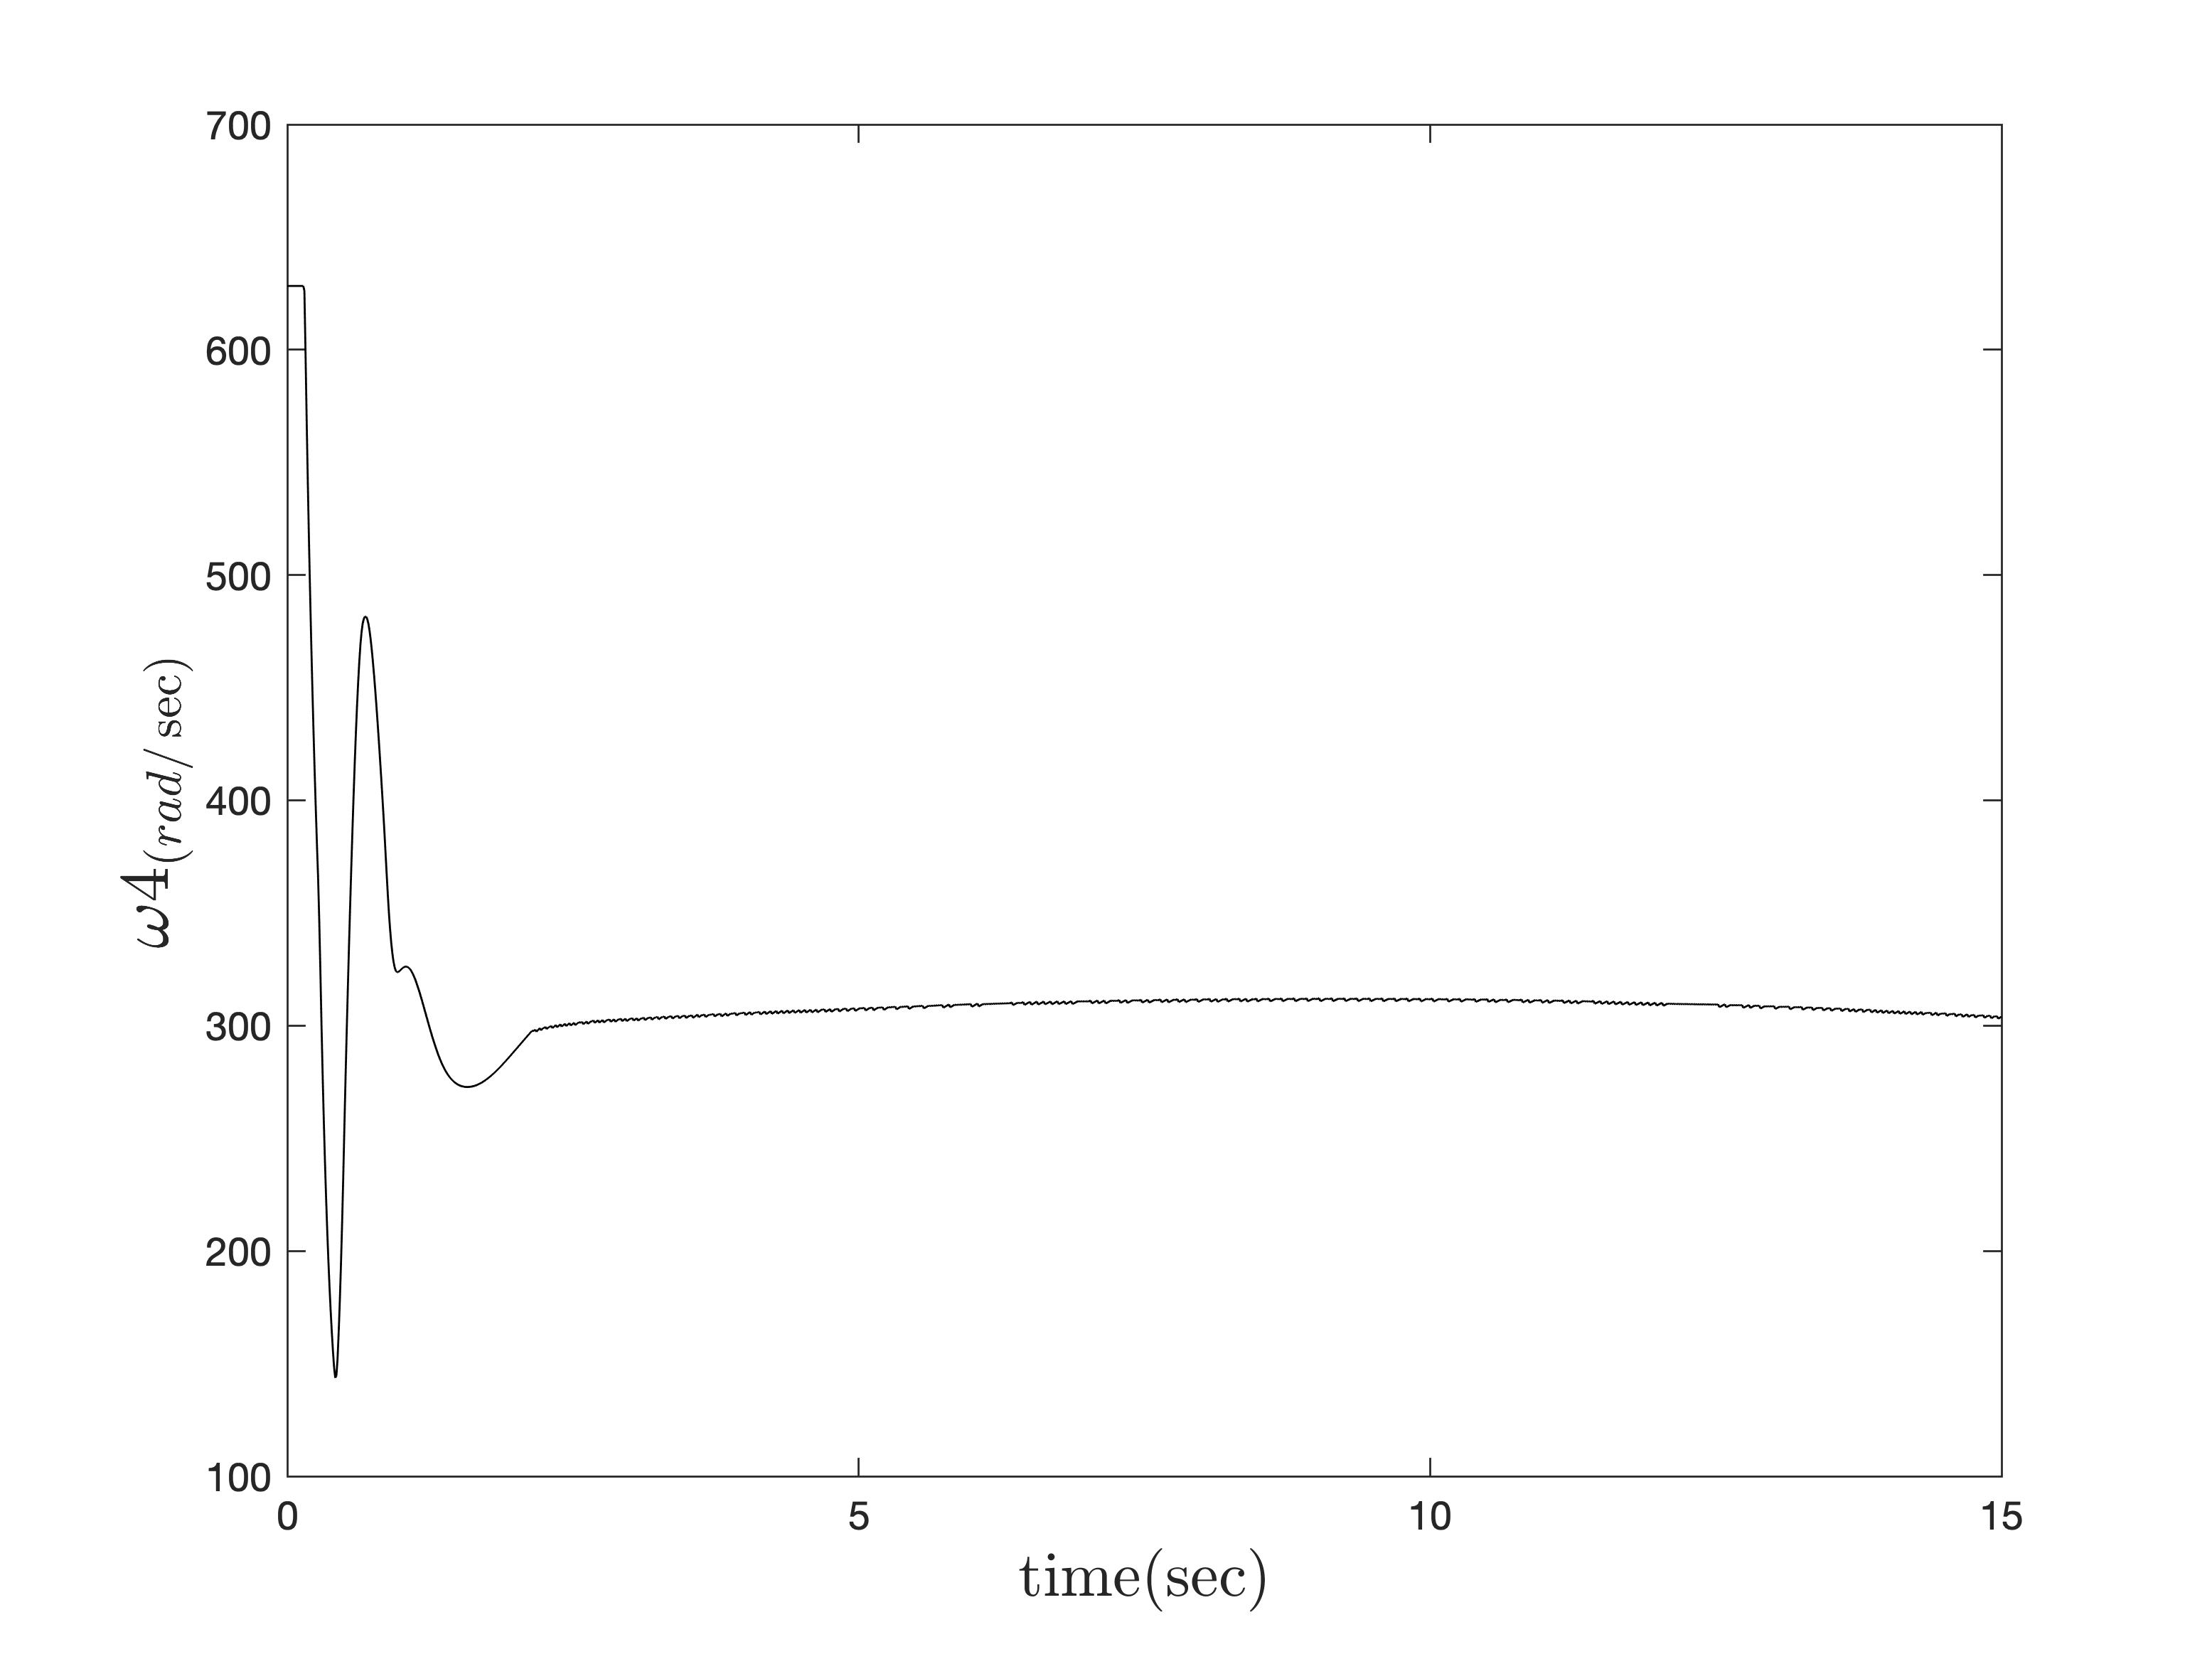
\includegraphics[width=.45\linewidth]{../Figures/MIL/LQIDG/MIMO/lqidg_roll_pitch_Omega4_nn.png}
	}
	\caption{‫‪فرمان کنترلی موتورها در کنترل وضعیت (تعقیب ورودی صفر)}
\end{figure}